\chapter{光波导与DFB激光器的基本理论}
\section{光波导理论分析}
在集成光学中,通常使用平面介质光波导来控制光波的传输,即负责光波从器件中的导入与导出,类似于电路中的导线。在很多应用中,波导又是光电子器件中重要的组成部分。可以这样说,平面光波导理论是集成光学的基础理论之一。结构最简单的平面光波导是由三层均匀介质组成的平板波导,如图\ref{fab_slab_waveguide}所示:

\begin{figure}[htb]
	\centering
	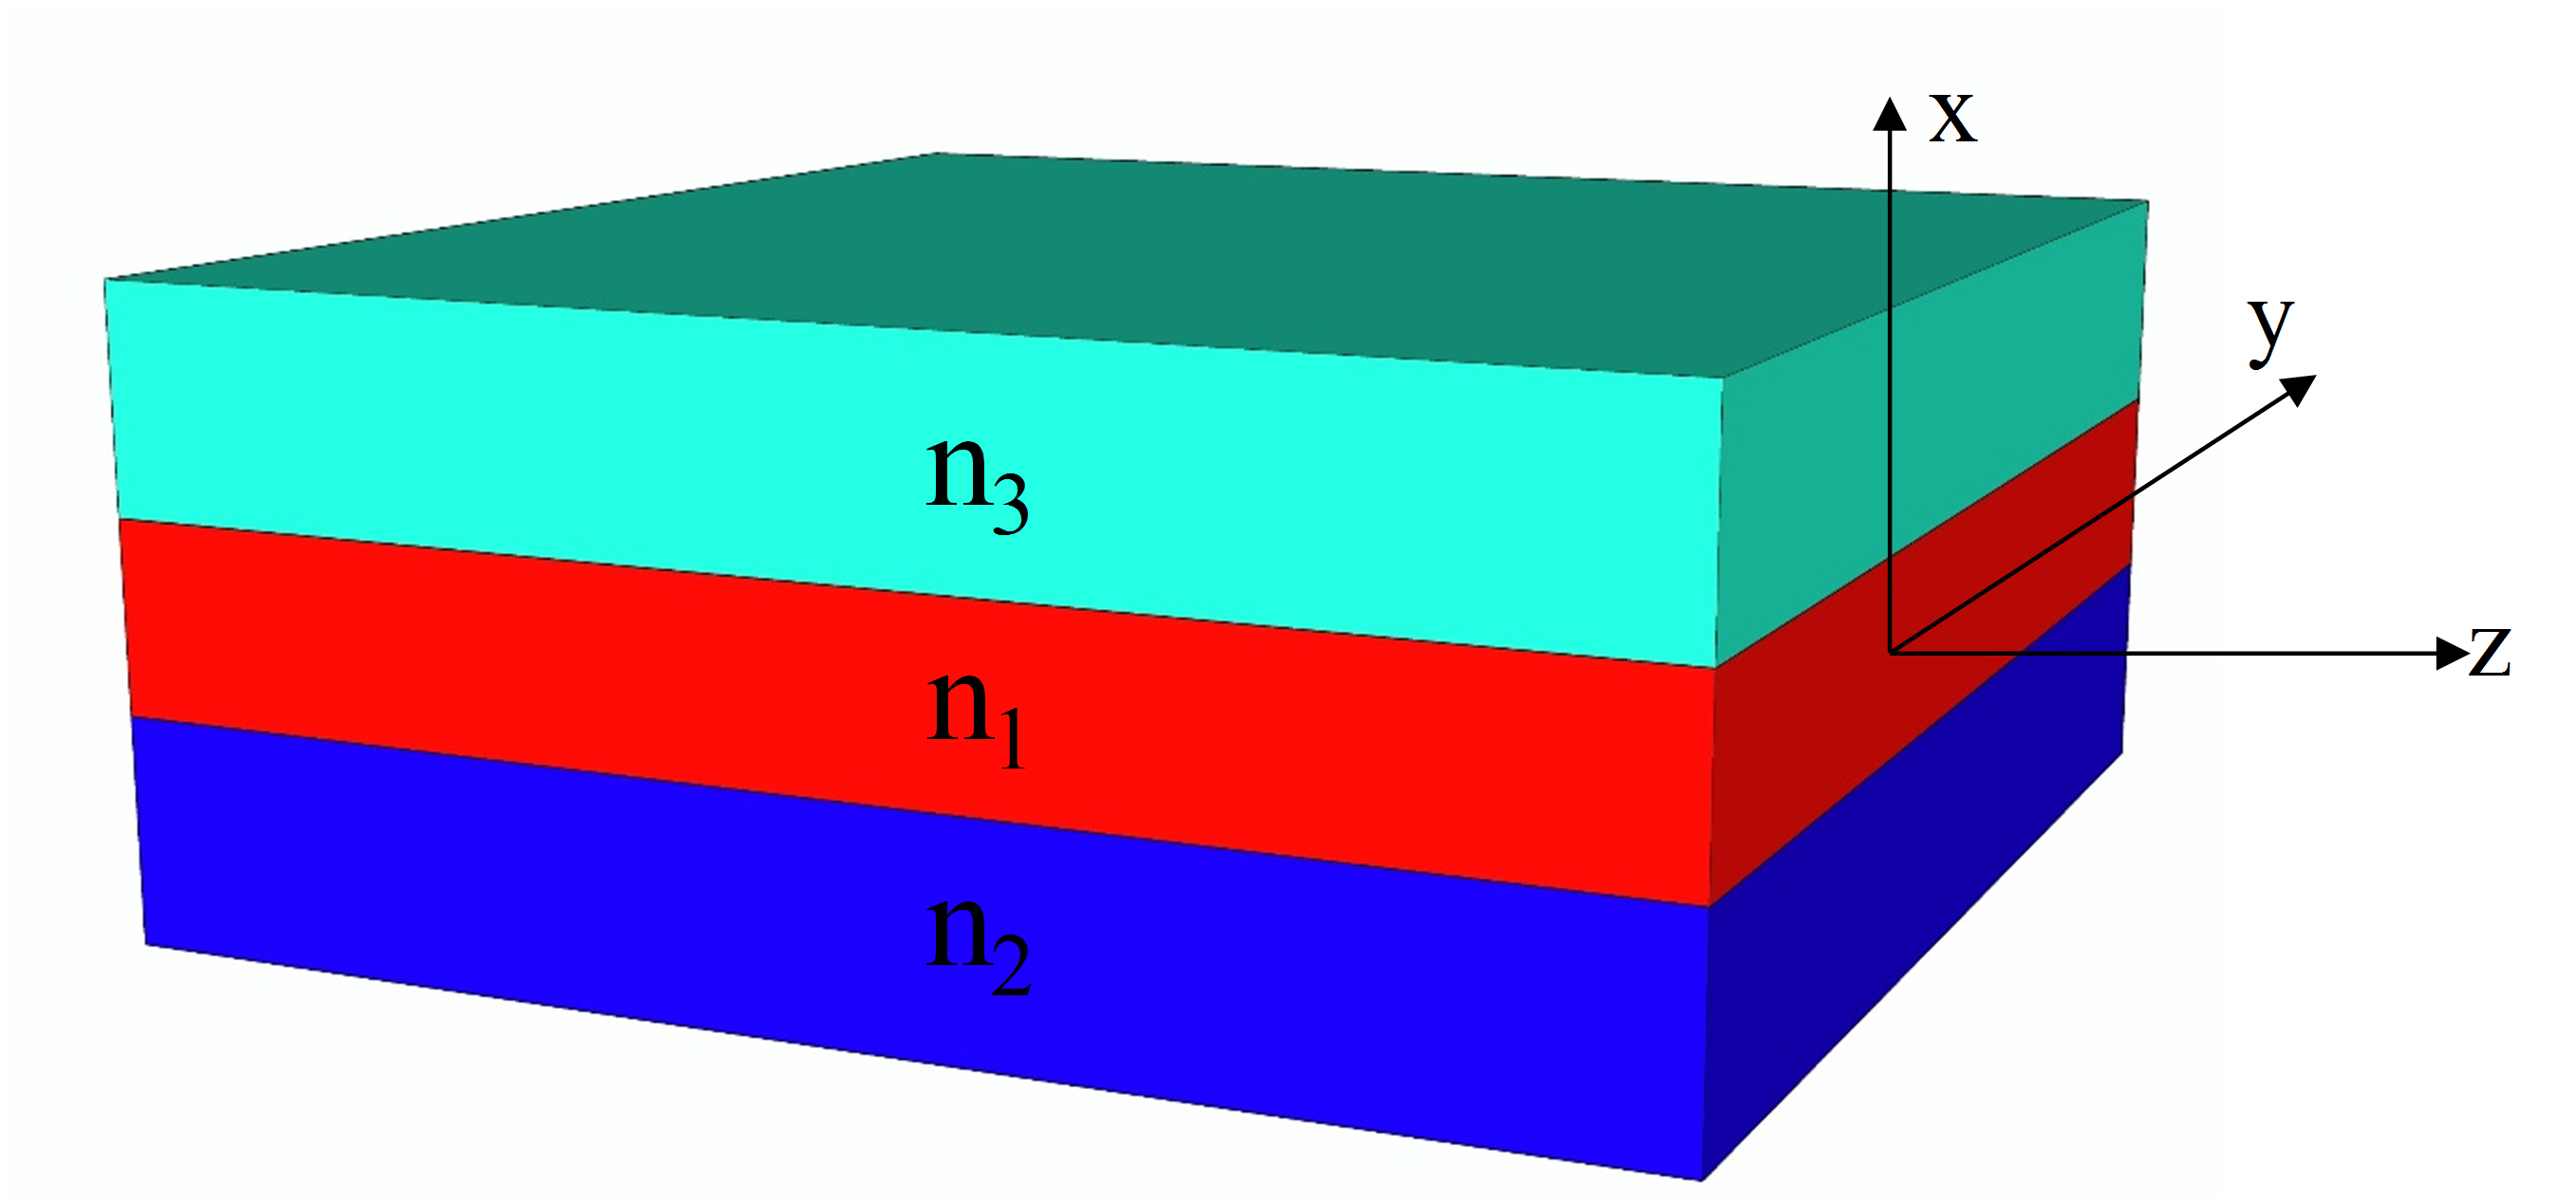
\includegraphics[width=12cm]{./Pictures/fab_slab_waveguide.jpg}
	\captionsetup{justification=centering}
	\caption{三层平板波导结构示意图}
	\label{fab_slab_waveguide}
\end{figure}

其中,为了保证光在波导中稳定传播,必须满足条件$n_{1}>max(n_{2},n_{3})$。该结构中间介质的折射率$n_{1}$最大,称为芯层;两侧介质的折射率较小,称为包层,理解平板波导的传输模式一般有射线光学和波动光学两种方式。射线光学方法对平板波导的模式传输解释通俗易懂,也能获得一些有价值的结论。但是当波导结构变复杂,比如条形波导、脊型波导,射线光学方法就无能为力了,为了对复杂波导的场分布、传输功率等问题进行分析,必须使用波动光学的方法,应用电磁场理论求解电磁波在介质波导这样一种特殊边界条件下的波动方程解,在此基础上再去分析传播模式的特性。

\subsection{波动方程}

要使用电磁场理论就不得不介绍麦克斯韦方程组,麦克斯韦在前人的电磁学研究成果基础上,总结推广了恒定和似穏电磁场的基本规律,提出了时变电磁场的传播规律,将它归纳为一组表达式,称之为麦克斯韦方程组。麦克斯韦方程组有微分和积分两种形式,微分形式的麦克斯韦方程组可以用来求解电磁场中某一处的场量,其表达式如公式\ref{maxwell1}~\~{}~\ref{maxwell4}所示:
\begin{equation}
\label{maxwell1}
\nabla \times \textbf{E} = -\dfrac{\partial\textbf{B}}{\partial t}
\end{equation}

\begin{equation}
\label{maxwell2}
\nabla \times \textbf{H} = \dfrac{\partial\textbf{D}}{\partial t}+\textbf{J}
\end{equation}

\begin{equation}
\label{maxwell3}
\nabla \cdot \textbf{D} = \rho
\end{equation}

\begin{equation}
\label{maxwell4}
\nabla \cdot \textbf{B} = 0
\end{equation}

式中,\textbf{D}、\textbf{E}、\textbf{B}、\textbf{H}分别表示电感强度(电位移矢量)、电场强度、磁感强度和磁场强度;$\rho$表示电荷密度;\textbf{J}表示传导电流密度;$\dfrac{\partial\textbf{D}}{\partial t}$表示位移电流密度,$\nabla$表示nabla算符,它既是微分算符,又是矢量。

在处理实际问题时,电磁场总是在媒质中传播的,所以我们需要物质方程来描述媒质对电磁场传播的影响。在静止的、各向同性媒质中,物质方程如下:

\begin{equation}
\label{constitutive_relations}
\left\{
\begin{array}{c}
\textbf{J}=\sigma\textbf{E}\\
\textbf{D}=\epsilon\textbf{E}\\
\textbf{B}=\mu\textbf{H}
\end{array}
\right.
\end{equation}
式中,$\sigma$是电导率,我们考虑介质波导的时候,$\rho=0$,$\sigma=0$;$\epsilon$是介电常数,在真空中$\epsilon=\epsilon_{0}=8.8542\times10^{-12}C^{2}/N\cdot m^{2}$,在介质中,$\epsilon=\epsilon_{0}\epsilon_{r}$,$\epsilon_{r}$为相对介电常数;$\mu$是磁导率,对于非磁性物质,$\mu_{r}=1$,$\mu=\mu_{0}\mu_{r}=4\pi\times10^{-7}N\cdot s^{2}/C^{2}$。

分别对公式\ref{maxwell1}和公式\ref{maxwell2}取旋度,利用公式\ref{constitutive_relations},并且令$v=1/\sqrt{\epsilon\mu}$,则\textbf{E}、\textbf{H}的方程化为:

\begin{equation}
\nabla^{2}\textbf{E}-\dfrac{1}{v^{2}}\dfrac{\partial^{2}\textbf{E}}{\partial t^{2}}=0
\end{equation}
\begin{equation}
\nabla^{2}\textbf{H}-\dfrac{1}{v^{2}}\dfrac{\partial^{2}\textbf{H}}{\partial t^{2}}=0
\end{equation}

考虑时谐电磁场,即$\textbf{E}=\textbf{E}_{0}e^{-i\omega t}$,$\textbf{H}=\textbf{H}_{0}e^{-i\omega t}$可以得到时谐波动方程,即本征频率问题:
\begin{equation}
\label{helmholtz1}
\nabla^{2}\textbf{E}+k^{2}\textbf{E}=0
\end{equation}
\begin{equation}
\label{helmholtz2}
\nabla^{2}\textbf{H}+k^{2}\textbf{H}=0
\end{equation}
其中,$k=k_{0}n=\omega \sqrt{\mu_{0}\epsilon}$,$k_{0}=\dfrac{2\pi}{\lambda_{0}}$为真空中的波矢,$\omega$为光波角频率,n是材料的折射率,c是真空中的光速,公式\ref{helmholtz1}~\~{}~\ref{helmholtz2}也被叫亥姆霍兹方程。

假设电磁场沿z轴方向传播时,沿z方向电磁场的变化可以用传输因子$e^{-j\beta z}$来表示,其中$\beta=k_{0}n_{eff}$为传播常数,$n_{eff}$为模式的等效折射率,即电磁场可以写成如下形式:
\begin{equation}
\label{betaz1}
\textbf{E}=\textbf{E}(x,y)e^{-i\beta z}
\end{equation}
\begin{equation}
\label{betaz2}
\textbf{H}=\textbf{H}(x,y)e^{-i\beta z}
\end{equation}

将公式\ref{betaz1}、\ref{betaz2}分别带入公式\ref{helmholtz1}、\ref{helmholtz2},则$\dfrac{\partial}{\partial z}$可以用$-j\beta$代替,$\dfrac{\partial^{2}}{\partial z^2}$可以用$-\beta^2$代替,从而可以得到直角坐标系下的矢量波动方程:
\begin{equation}
\label{helmholtz3}
\left(\dfrac{\partial^2}{\partial x^2}+\dfrac{\partial^2}{\partial y^2}\right)\textbf{E}(x,y)+(k_0^2n^2-\beta^2)\textbf{E}(x,y)=0
\end{equation}
\begin{equation}
\label{helmholtz4}
\left(\dfrac{\partial^2}{\partial x^2}+\dfrac{\partial^2}{\partial y^2}\right)\textbf{H}(x,y)+(k_0^2n^2-\beta^2)\textbf{H}(x,y)=0
\end{equation}

在实际求解过程中,光有亥姆霍兹方程的解会有无穷多组,还要考虑边界条件得到具有实际物理意义的解。利用波动方程\ref{helmholtz3}、\ref{helmholtz4}以及边界条件,可以得到一系列波导的本征模式解,它们具有如下特性:
\begin{enumerate}[(1)]
	\item 
	色散性~~~~不同的本征模式有不同的等效折射率$n_{eff}$,其各自沿传播方向有一个等效的传播相速度$v_{eff}=c/n_{eff}$
	\item 
	正交性~~~~不同本征模式间的场分布叠加积分为零,意味着在沿传播方向均匀的波导中,本征模式之间不存在串扰。
	\item 
	完备性~~~~任意能在介质波导中稳定传输的光场都可以分解为本征模式的线性叠加,光场的传播特性由这些本征模式的特性所决定。
\end{enumerate}

综上,我们可以通过研究波导各本征模的特性,就可以知道任意稳定传输光场的传播特性。故对本征模式模场分布和等效折射率的求解计算便成了设计、分析波导结构的基础与关键。

\section{光波导的数值计算方法}

对于如图\ref{fab_slab_waveguide}所示的平板波导,可以利用解析的方法得到其本征模式的特征方程\cite{ttt2005jcgx}。但是当电磁场在平板波导中传输时,在无约束的方向上会发散,这不利于器件的集成,为了避免这种情况,集成光学中常使用的三维波导结构如图\ref{fab_strip_waveguide}所示:

\begin{figure}[htb]
	\centering
	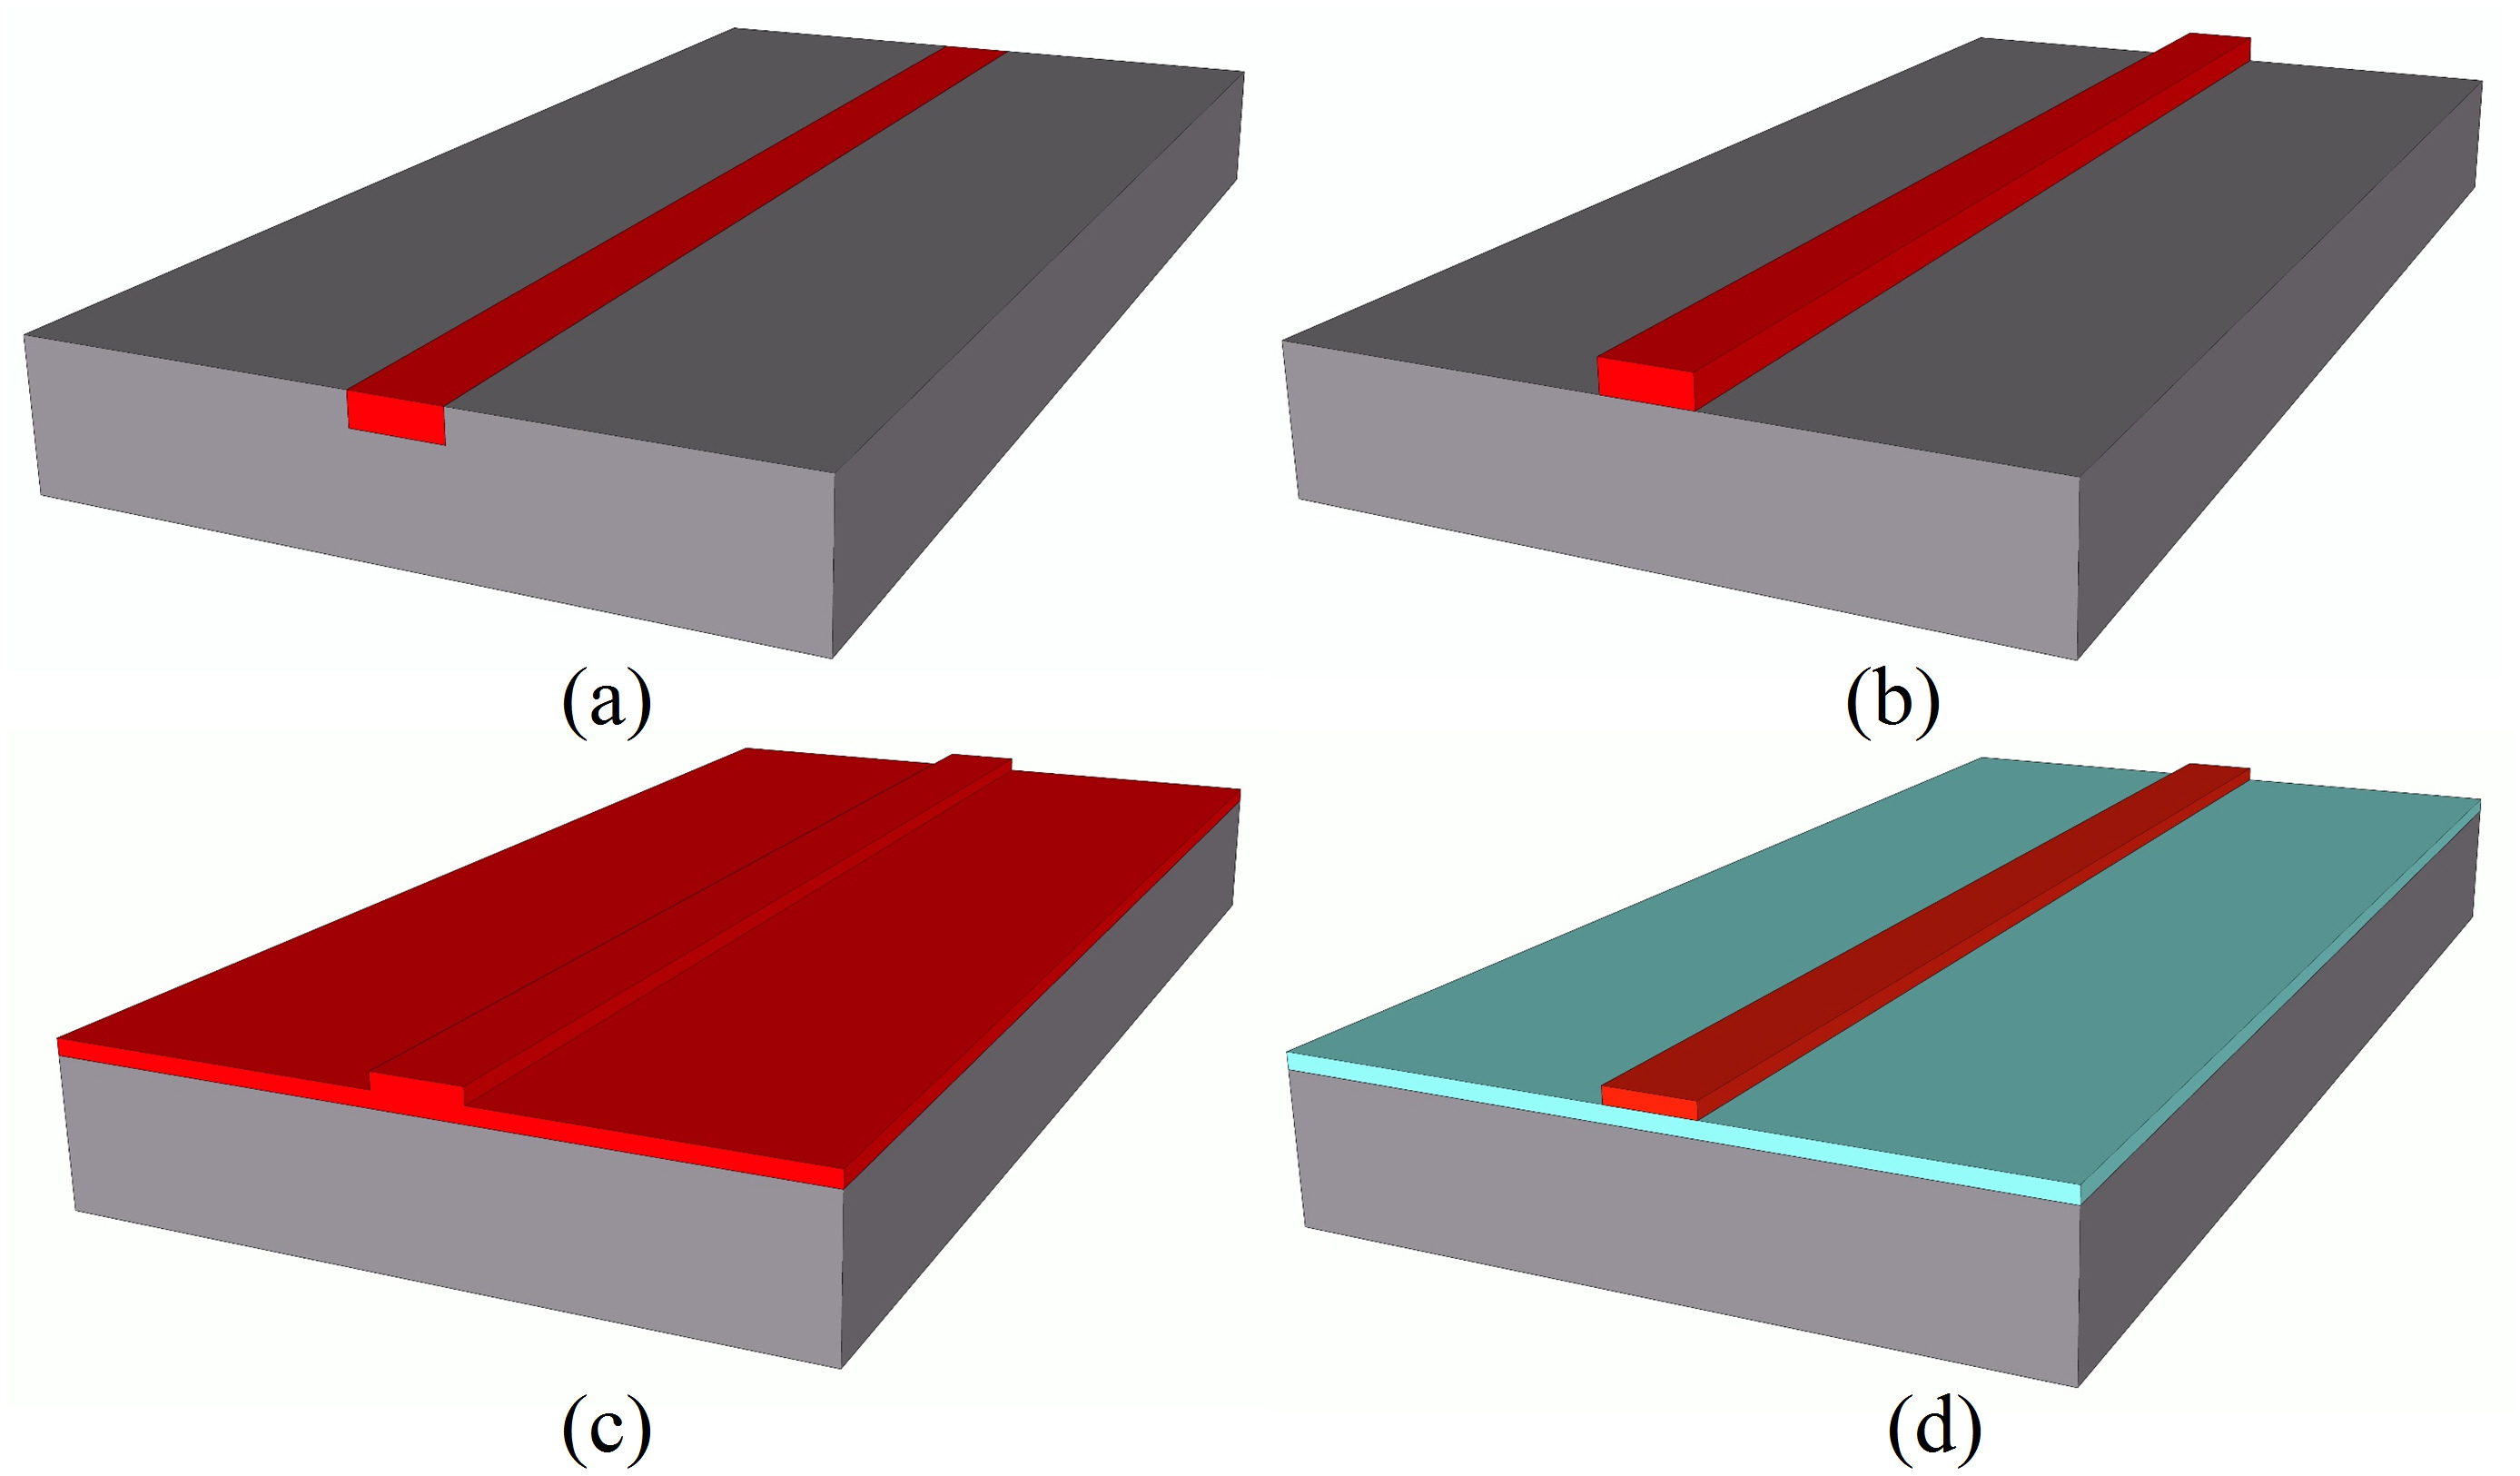
\includegraphics[width=13cm]{./Pictures/fab_strip_waveguide.jpg}
	\captionsetup{justification=centering}
	\caption{几种常见的光波导结构:(a)掩埋型;(b)条带型;(c)脊型;(d)条载型}
	\label{fab_strip_waveguide}
\end{figure}

三维波导与二维平板波导不同,没有严格的解析模式解,只能用近似分析法或者数值方法求解。在弱导近似下,主要模式光能基本被限制在芯层波导中传输,这时三维波导中存在的不再是TE模式或者TM模式,而存在以$E_y$、$H_x$为主的$E_{mn}^y$模式(或称为似TE模)和以$H_y$、$E_x$为主的$E_{mn}^x$模式(或称为似TM模)。模式的上标x、y表示电场矢量的偏振方向(坐标系与图\ref{fab_slab_waveguide}一样),下标m、n为模式序号,代表场量在x轴和y轴方向出现场量最大值的个数。与平板波导波导相比,条形波导的分析要复杂的多,通常使用的近似分析法有Marcatili方法和等效折射率法\cite{okamoto2006fundamentals}。但是得益于现在计算机计算能力的提升,我们很少需要用到这两种方法去近似求解亥姆霍兹方程,采用的往往是用数值方法进行模拟计算,只要数值离散足够精细,就能获得非常精确的结果。常见的本征模式数值求解法主要有有限差分法(finite difference method, FDM)\cite{stern1988semivectorial}和有限元法(finite element method, FEM)\cite{jin2015finite}两种。该两种方法的核心思想都是将连续问题离散化,进而转化为有限形式的线性方程组进行数值求解,其过程大致可以分为以下两步:1、对求解区域进行网格划分,其中FDM采用的是矩形网格,而FEM一般采用三角形的网格。2、用差分方程代替微分算子,将偏微分方程的求解问题转化为有限个线性代数方程组的求解问题。相对于FEM,FDM方法容易理解、效率较高,但是FEM由于网格划分比较灵活,具有更好的适应性和精度。商用软件Lumerical Mode Solutions\cite{modesolution}采用FDM,COMSOL\cite{comsol}则采用FEM。

\subsection{时域有限差分法}

在实际的平面集成光器件的设计过程中,计算出模式的分布往往还不够,我们需要计算光场的传输,常用的方法有光束传播方法(beam~propagation~method,~BPM)\cite{van1981beam},本征模式展开法(eigenmode~expansion,~EME)\cite{gallagher2003eigenmode},时域有限差分法(finite~difference~time~domain,~FDTD)\cite{yee1966numerical}。光束传播方法(BPM)由于采用了标量近似和傍轴近似,因此无法获得模式的偏振和反射信息且只能仿真光场沿光轴缓慢变化的情况,这对于基于SOI的集成光学器件仿真是不适用的。本征模展开法(EME)虽然是一种全矢量、双向的算法,且能够计算大角度的光场传输,但是其是在频域求解麦克斯韦方程组,故其每次只能进行单频率点的仿真。时域有限差分法(FDTD)是一种能够精确求解任意结构中麦克斯韦方程组的算法,其直接对麦克斯韦方程组进行离散化,仿真区域被离散成一个个Yee元胞,除了将连续的物理空间用离散的空间格点所引入的近似以外,没有引入其他任何的近似。由于FDTD是基于时域的算法,其经过一次仿真,经过傅里叶变换之后就可以得到一段频谱范围内的响应。FDTD是1966年的时候由Yee博士首次提出的,随后经过很多人的改进,如今已经被广泛应用到诸如太阳能电池的设计、CMOS图像传感器设计、超材料设计、集成光电子器件设计等电磁学的各个领域。

\begin{figure}[htb]
	\centering
	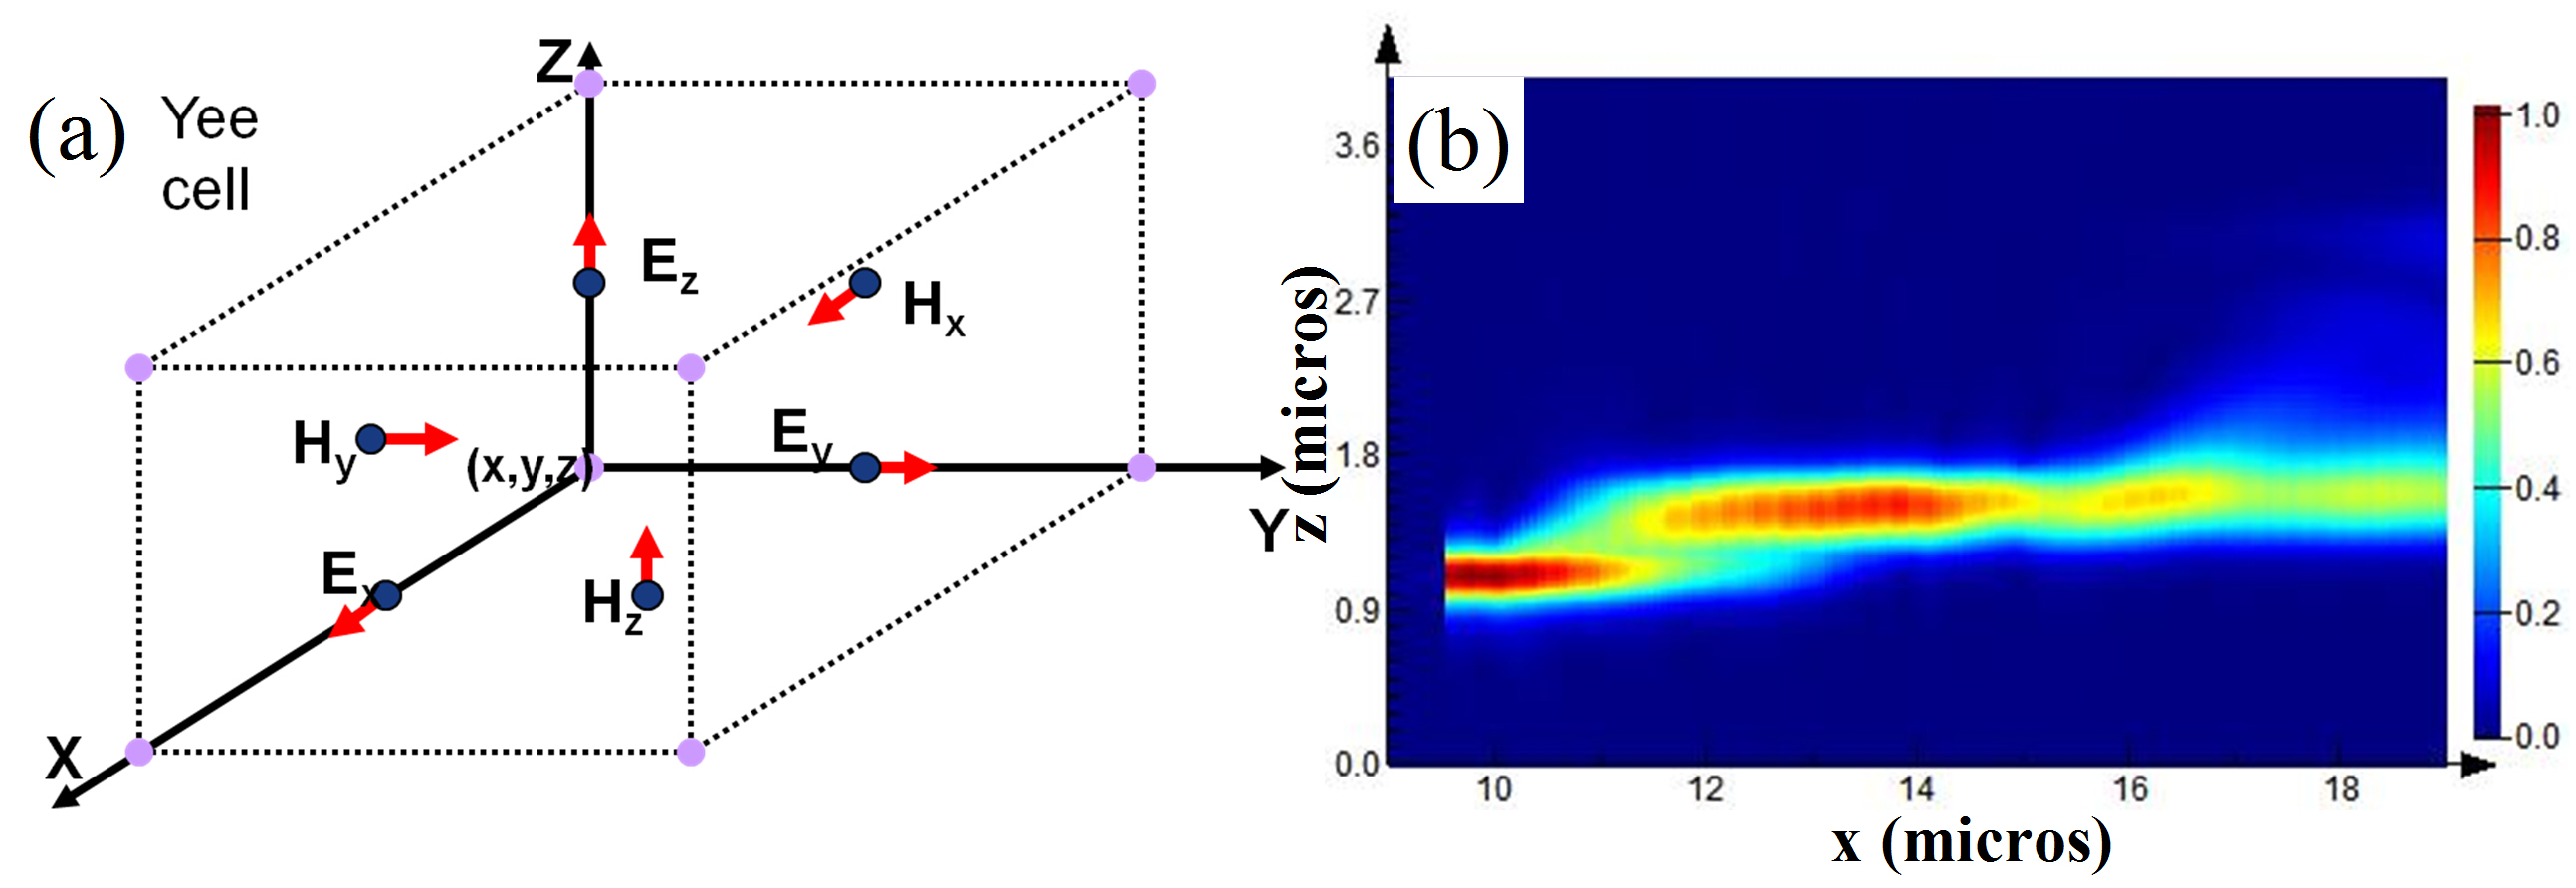
\includegraphics[width=16cm]{./Pictures/fab_yeecell.jpg}
	\captionsetup{justification=centering}
	\caption{(a)三维直角坐标系下的Yee网格的分布图\cite{fdtdsolution};(b)~FDTD算法计算得到的光场传输图}
	\label{fab_yeecell}
\end{figure}

图\ref{fab_yeecell}(a)所示为直角坐标系下的Yee网格示意图,其中电场分量位于网格单元每条棱的中心点处,磁场分量位于网格单元的每个面中心,这种电、磁场分量交叉分离划分的方法能够确保它们各自的分量在介质分界面处连续,而且利用这种网格划分方法,不但可以实现方程在三维空间中的差分运算,而且也同时满足了安培环路积分定律和法拉第电磁感应定律。因此利用该种网格划分方法对空间进行离散化,可以准确地被用来模拟电磁场在介质波导中的实际传输过程。图\ref{fab_yeecell}(b)为本文利用FDTD计算垂直耦合结构的耦合效率时得到的光场传输图。

\section{DFB激光器的基本原理}

激光器产生激射的三个条件分别是:1增益介质,2谐振腔,3泵浦源。谐振腔通过把一部分光周期性地反射回原来的地方,对于某些波长来说刚好满足干涉增强的条件,并通过被泵浦的增益介质实现受激放大,从而产生激光\cite{numai2015fundamentals,suhara2004semiconductor}。

对于半导体激光器来说,当导带中的电子与价带中的空穴复合时,就会产生光子。该过程中需要满足能量守恒与动量守恒。能量守恒决定了出射光子的能量,其等于电子与空穴所处能级的能量差。动量守恒决定了只有直接带隙半导体才能比较高效地发光。常用的直接带隙材料包括AlGaAs,InGaAs和InGaAsP,其带隙可以通过改变不同元素的组分进行调节,从而可以控制激光器的激射波长。

对于最简单的FP(Fabry-Perot)激光器来说,谐振腔由两个解理的端面组成,FP激光器的优点是结构简单,但由于材料的增益谱往往比较宽,会覆盖多个FP腔的纵模,故其出射为多纵模,使得其不适用于光通信系统,因为多个波长的存在会加剧光纤的色散影响。如图\ref{fab_fp_laser}所示FP激光器激射模式示意图,每个纵模的波长满足谐振条件:
\begin{equation}
m\lambda = 2n_e(\lambda)L
\end{equation}
其中$L$为激光器的腔长,$n_e(\lambda)$为等效折射率。

\begin{figure}[htb]
	\centering
	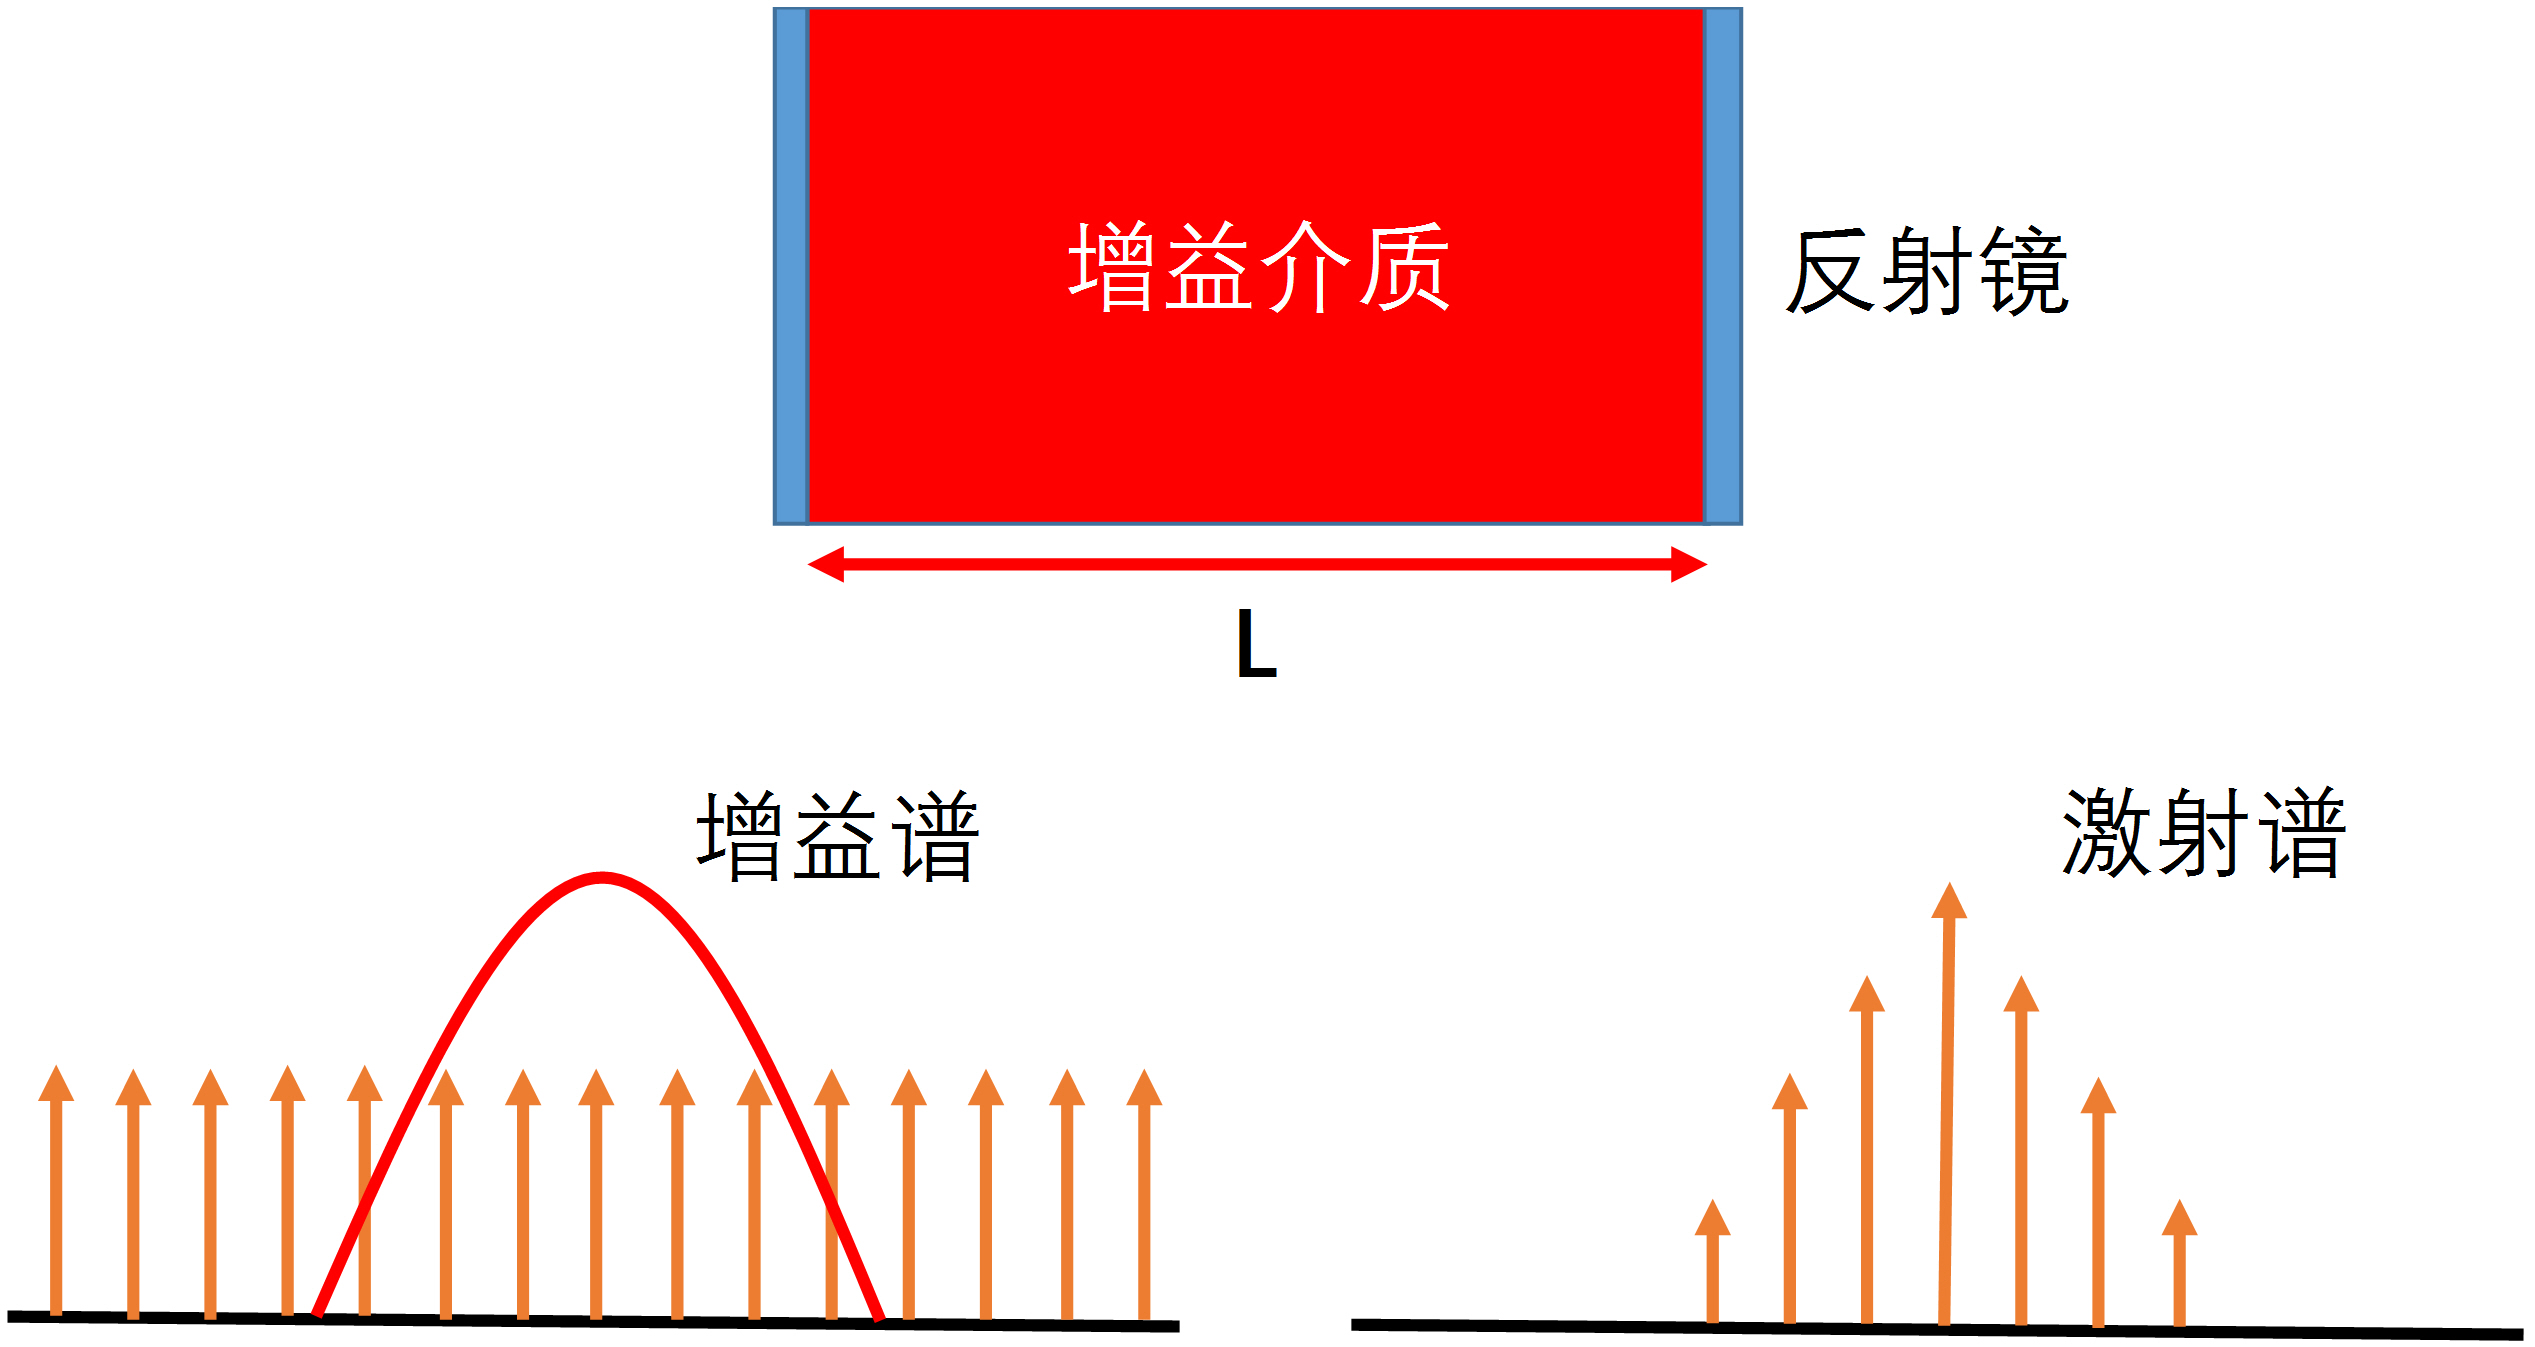
\includegraphics[width=12cm]{./Pictures/fab_fp_laser.jpg}
	\captionsetup{justification=centering}
	\caption{FP激光器激射模式示意图}
	\label{fab_fp_laser}
\end{figure}

DFB激光器通过将FP激光器中由两面反射镜构成的简单谐振腔替换成分布反馈布拉格反射镜,可以克服FP激光器的多模问题,只出射一个纵模,其激射模式示意图如图\ref{fab_dfb_laser}所示。分布反馈布拉格光栅可以通过周期性地改变波导的宽度或者厚度来实现,从而周期性地改变波导的等效折射率。当光经过布拉格光栅时,在每个折射率突变的界面都会产生反射,使得前向传输的光与背向传输的光相互耦合。由于分布反馈布拉格光栅的周期往往只有几百纳米,故其产生的自由频谱范围(free spectral range, FSR)较大,可以在增益介质的增益带宽内实现单纵模激射。对于DFB激光器来说,可以通过改变分布反馈布拉格光栅的周期和等效折射率来改变激射波长。

\begin{figure}[htb]
	\centering
	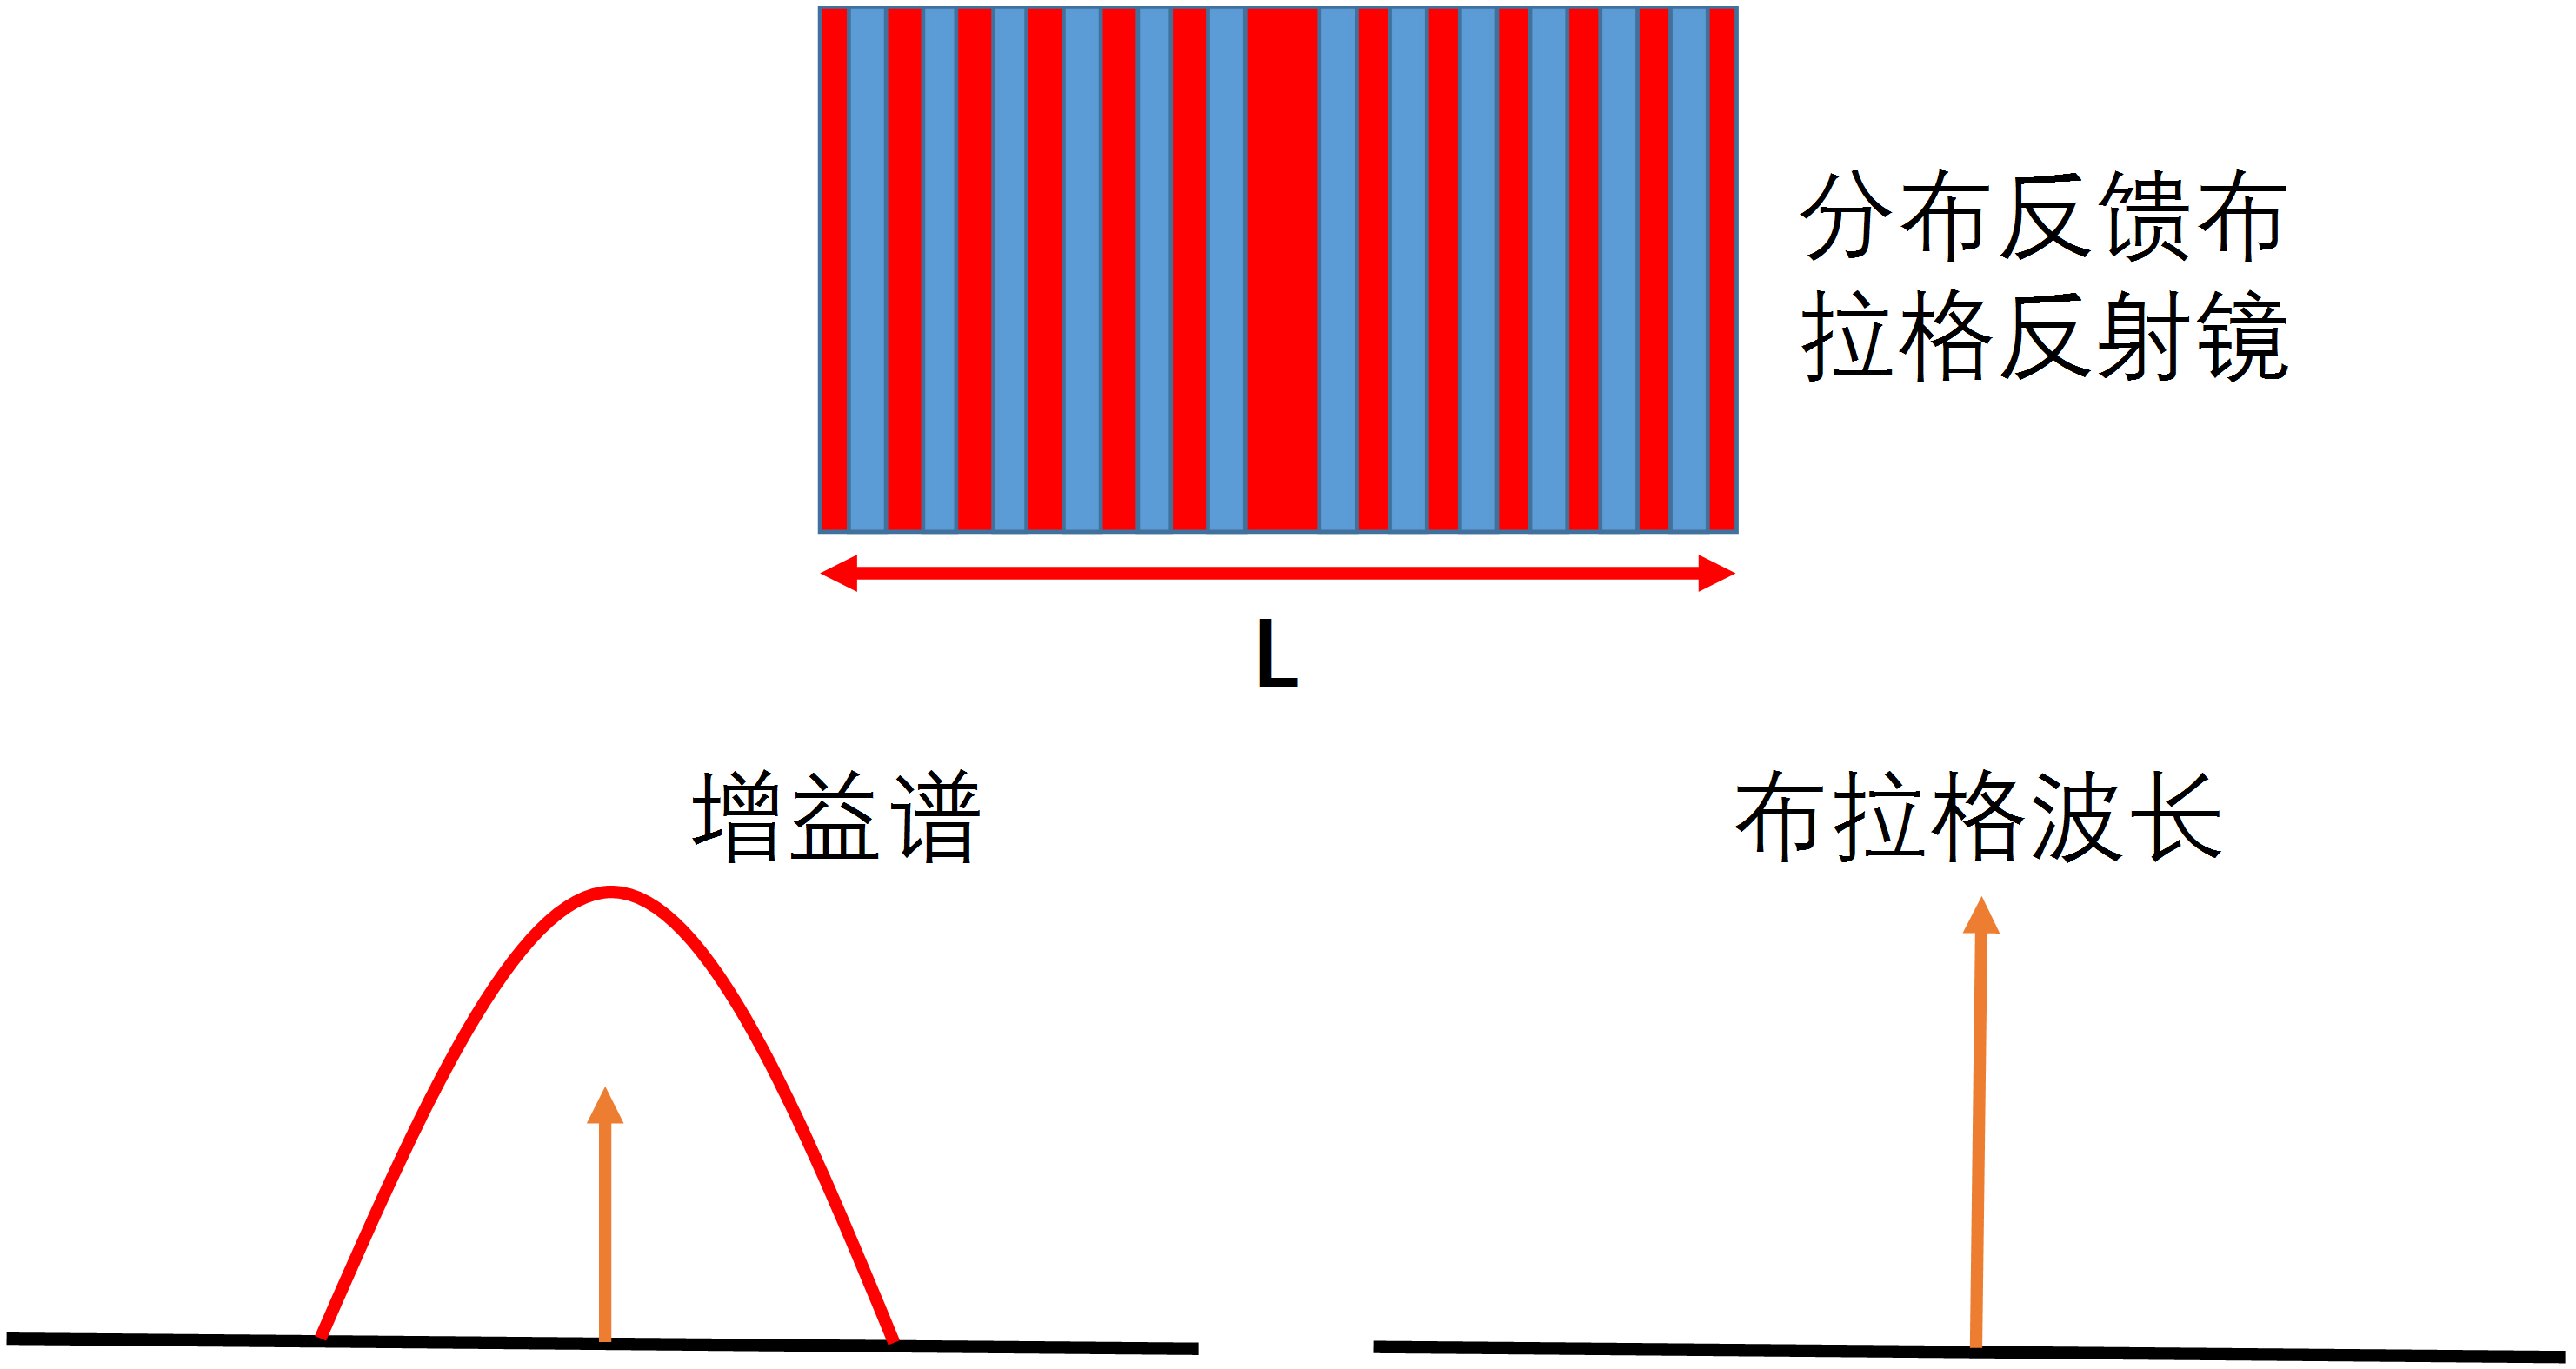
\includegraphics[width=12cm]{./Pictures/fab_dfb_laser.jpg}
	\captionsetup{justification=centering}
	\caption{$\lambda/4$相移DFB激光器激射模式示意图}
	\label{fab_dfb_laser}
\end{figure}

DFB激光器最早由Kogelnik和Shank在上世纪70年代提出\cite{kogelnik1971stimulated,kogelnik1972coupled},然后由Nakamura等人首先在GaAs平台上实现了光泵浦的DFB激光器\cite{nakamura1973optically},之后他们利用双异质结结构在GaAs-GaAlAs平台上实现了电泵浦的DFB激光器\cite{nakamura1974gaas},但这都需要液氮制冷。直到分离限制异质结结构(separate~confinement~heterostructure,~SCH)的提出,Nakamura等人才在GaAs-GaAlAs平台上实现了室温下的连续工作的DFB激光器\cite{nakamura1975cw}。从这以后,DFB激光器吸引了许多研究人员的关注并由于其优异的性能成为了光通信中最主要的光源。为了更深刻理解DFB激光器的工作原理,需要利用速率方程和耦合模理论这两个模型。

\subsection{速率方程}

\subsubsection{载流子密度速率方程}
典型的半导体激光器的截面图如图\ref{laser_activelayer}所示,电流注入端通常采用高掺杂使其与金属形成欧姆接触,有源区不进行掺杂以减小波导的损耗。有源区的载流子密度可以用连续性方程(continuity equations)来描述:
\begin{equation}
\label{continuity_equation}
\left\{
\begin{array}{l}
\dfrac{\partial N(x,y,z,t)}{\partial t} = \dfrac{1}{q}\nabla\cdot J_{n}+G-U\\
\dfrac{\partial P(x,y,z,t)}{\partial t} = -\dfrac{1}{q}\nabla\cdot J_{p}+G-U
\end{array}
\right.
\end{equation}
其中,$J_{n}$和$J_{p}$分别是电子和空穴产生的电流密度,$G$是载流子产生的速度,$U$是载流子复合的速度。对于由折射率差形成有源层波导的激光器来说,我们可以假设电流只在垂直方向传导,在水平方向是均匀的,且由于有源区具有电中性的特点,电子产生的电流应该跟空穴产生的电流相等,故公式\ref{continuity_equation}可以简化为:

\begin{figure}[htb]
	\centering
	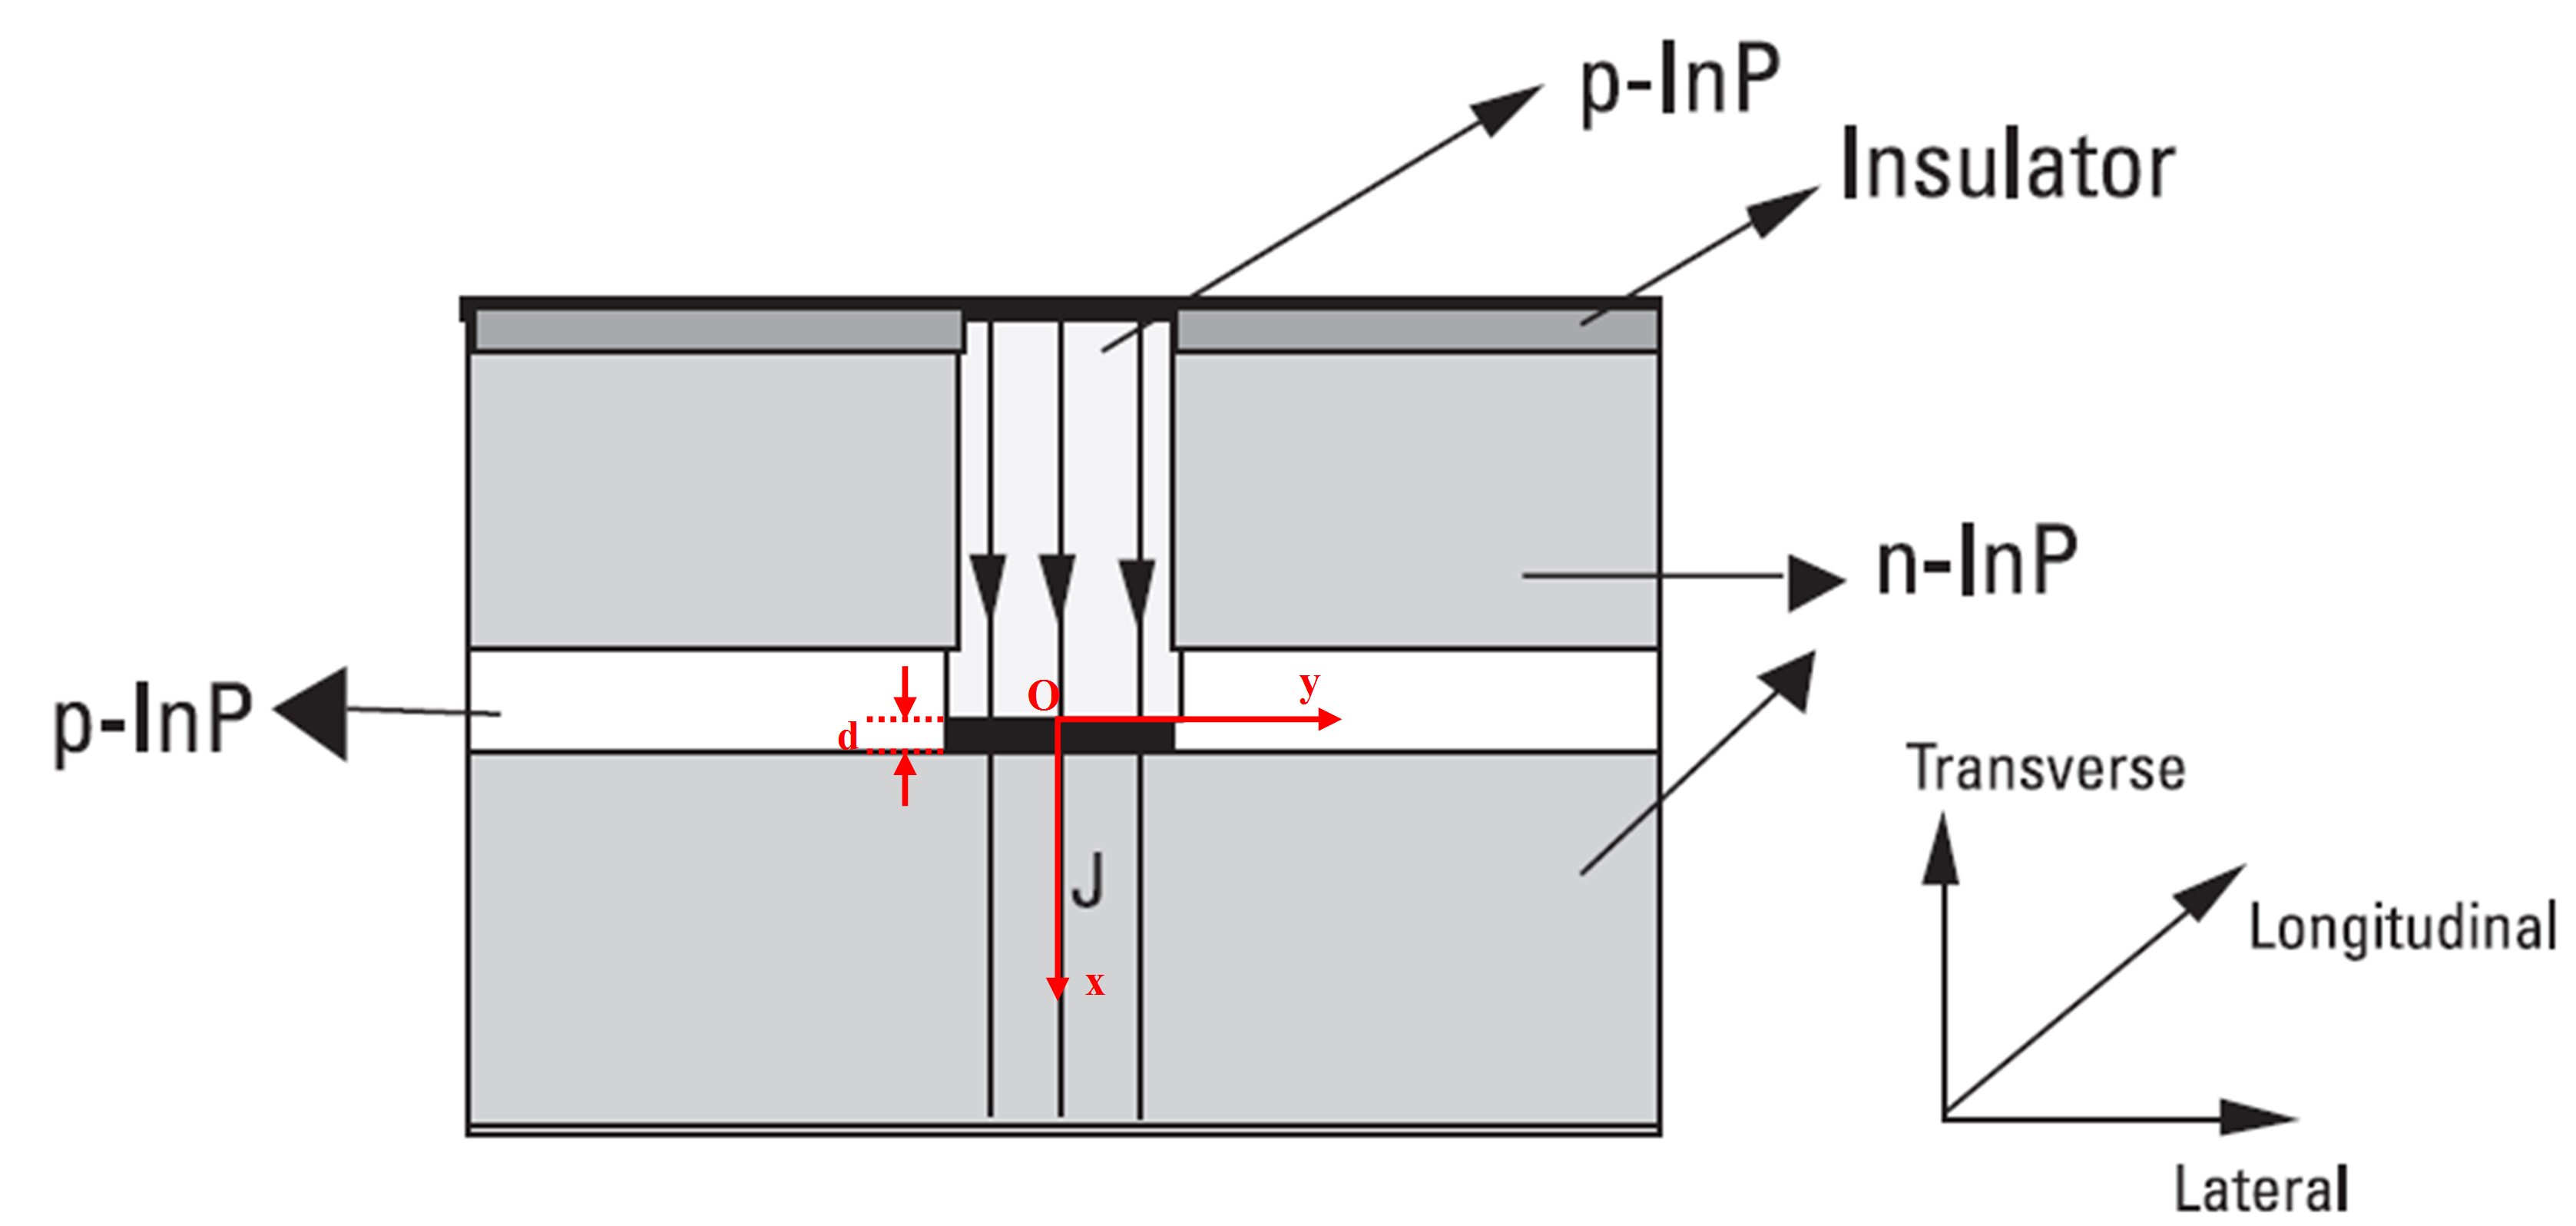
\includegraphics[width=14cm]{./Pictures/laser_activelayer.jpg}
	\captionsetup{justification=centering}
	\caption{典型半导体激光器的截面图\cite{morthier2013handbook}}
	\label{laser_activelayer}
\end{figure}

\begin{equation}
\label{continuity_equation_simplified}
\begin{array}{l}
\dfrac{\partial N(x,y,z,t)}{\partial t} = \dfrac{1}{q}\dfrac{\partial J_{n}}{\partial x}+G-U\\
N = P ~~\text{且}~~ \dfrac{\partial J_{p}}{\partial x} = -\dfrac{\partial J_{n}}{\partial x}~~(0 \le x \le d)
\end{array}
\end{equation}

其中,$x$为垂直的横向方向,原点取有源层波导的上边缘中点,$x$轴的正方向朝下,$d$为有源层的厚度。将公式\ref{continuity_equation_simplified}在有源层进行平均处理,得到平均载流子密度$N$:

\begin{equation}
\label{average_carrier_density}
\dfrac{\partial N}{\partial t} = \dfrac{1}{qd}[J_{n}(d)-J_{n}(0)]+(G-U)_{av}
\end{equation}

其中,$J_{n}(d)$是有源层与n-InP边界处电子产生的电流,$J_{n}(0)$是有源层与p-InP边界处电子产生的电流。由于n-InP有比有源区更大的能带间隔,所以空穴不会从有源区泄漏到n-InP中,同理,电子也不会泄漏到p-InP中,故$J_{n}(d)=J(d)=J$,$J_{n}(0)=0$。如果再将载流子复合,其中包括自发复合和受激辐射复合一起考虑进来,我们最终可以得到载流子的速率方程为:

\begin{equation}
\label{carrier_density_rate_equation}
\dfrac{\partial N}{\partial t} = \dfrac{J}{qd}-AN-BN^{2}-CN^{3}-\sum_{m}G(N,\lambda_{m})S_{m}
\end{equation}

其中,第一项代表有源区载流子的注入并且假设注入效率是100\%;$AN$代表载流子通过表面态或者陷阱产生的自发复合,因为该过程中只有一个载流子参与,故其复合速度与载流子的浓度成正比\cite{shockley1952statistics};$BN^{2}$代表自发辐射复合,因为该过程需要有两个载流子参与,故其复合速度与载流子浓度的平方成正比\cite{olshansky1984measurement};$CN^{3}$代表俄歇复合,电子与空穴复合的能量被另一个电子或者空穴吸收,因此该过程需要有三个载流子参与,故其复合速度与载流子浓度的三次方成正比\cite{agrawal1986long}。俄歇复合的强度与半导体的禁带宽度($E_{g}$)密切相关,$E_{g}$越小,俄歇复合速率就越大,所以俄歇复合对长波长的激光器影响更为严重\cite{dexiu1999};$\sum_{m}$项代表受激辐射复合,求和符号中的$m$代表对所有模式的求和,受激辐射速率与模式的平均光子密度$S_{m}$和增益系数$G(N,\lambda_{m})$成正比。增益系数除了与载流子浓度($N$)和波长($\lambda$)相关外,还与不同模式中的的光子密度($S_{m}$)相关,所以增益系数一般会在光子密度达到一定程度的时候饱和。

\subsubsection{光子密度速率方程}
光子密度速率方程可以根据不同模式中的光子数守恒得到,影响光子密度的过程主要有两个,一是光子的产生,包括受激辐射和自发辐射,二是光子的损耗,包括材料的吸收和反射镜的损耗。其中,受激辐射和损耗与平均光子密度成正比,自发辐射与光子数密度无关,而与载流子密度相关,故光子密度速率方程可以表示为\cite{petermann2012laser}:

\begin{equation}
\label{photon_density_rate_equation}
\dfrac{\partial S_{m}}{\partial t} = [G(N,\lambda_{m})-\gamma_{m}]S_{m}+\dfrac{R_{sp}}{V_{act}}
\end{equation}

其中,$G(N,\lambda_{m})$表示模式增益,对应受激辐射,其与载流子密度和波长相关,$R_{sp}$代表单位时间内耦合进入模式$m$的自发辐射光子数,$S_{m}$代表模式$m$的光子密度,单位为$cm^{-3}$,$\gamma_{m}$代表模式$m$总的损耗,主要包括内部吸收损耗和反射镜损耗:

\begin{equation}
\label{photon_loss}
\gamma_{m} = \gamma_{int}+\gamma_{fac,m} = V_{g,m}(\alpha_{int}+\alpha_{fac,m})
\end{equation}
其中,$\alpha_{int}$是单位长度($cm$)的吸收损耗,$\alpha_{fac,m}$则是模式$m$在两个端面总的损耗,$V_{g,m}$则是对应模式的群速度。

\subsubsection{相位条件}

我们以FP激光器作为例子来简要介绍激光器在谐振时需要满足的相位条件,所得到的结果对DFB激光器也具有参考意义。当光波满足在谐振腔内往返一周所经历的相位变化为2$\pi$的整数倍时,该波长才能满足激射条件。相位条件可以用公式\ref{phase_equation}表达:

\begin{equation}
\label{phase_equation}
2\dfrac{\omega_{m}}{c}n_{eff}(N,\omega_{m})L = 2m\pi
\end{equation}

其中,$m$代表不同的模式,为整数;$L$表示腔长;$\omega_{m}$表示模式的角频率;$n_{eff}$表示模式的等效折射率,其与载流子浓度$N$和角频率$\omega_{m}$相关。将两边同时对$\omega$和$N$微分,公式\ref{phase_equation}可以化为:

\begin{equation}
\label{phase_equation_diff}
\Delta\omega_{m} n_{eff} + \omega_{m} \dfrac{\partial n_{eff}}{\partial \omega} \Delta\omega_{m}+\omega_{m}\dfrac{\partial n_{eff}}{\partial N} \Delta N = 0
\end{equation}

据此,可以得到$\Delta\omega_{m}$与$\Delta N$的关系为:

\begin{equation}
\label{frequency_carrier_relation}
\Delta\omega_{m} = -\dfrac{\omega_{m}}{c}v_{g}\dfrac{\partial n_{eff}}{\partial N} \Delta N = \dfrac{\alpha}{2}\dfrac{\partial G(N,\lambda_{m})}{\partial N} \Delta N 
\end{equation}

公式\ref{frequency_carrier_relation}表示了谐振角频率的偏移量与载流子浓度变化的关系,第二个等式引入的参数$\alpha$,表示线宽增强因子,其与材料和波长相关,通常值为1\~{}5。第二个等式中增益对载流子浓度的微分$\dfrac{\partial G(N,\lambda_{m})}{\partial N}$称为微分增益,通常值为0.5\~{}2 $\times$ 10\SP{18} $cm^{-3}$。

\subsubsection{光学增益}

公式\ref{photon_density_rate_equation}中的模式增益$G(N,\lambda_{m})$与材料增益成正比:
\begin{equation}
\label{modal_gain}
G(N,\lambda_{m}) = \Gamma g(N,\lambda_{m})\nu_g = g_{mod}\nu_g
\end{equation}
其中,$\Gamma$是模式的限制因子,即模式的能量在增益区中所占的比例。$g_{mod}$表示单位距离的增益,乘以群速度$\nu_g$之后就变成了单位时间的增益。

经过前人在理论和实验上的验证,对于体材料来说,其增益与载流子密度成线性关系:
\begin{equation}
\label{bulk_material_gain_equation}
g(N,E) = A(E)N-B(E)
\end{equation}
公式中将$E$取代前面的$\lambda$表示是为了作图的方便,$A(E)$为微分增益,通常值为1\~{}5~$\times$~10\SP{16}~$cm^{2}$,B(E)与透明载流子密度相关,$N_t(E)=B(E)/A(E)$。图\ref{bulk_material_gain}给出了激射波长在1550~$nm$的体材料InGaAsP激光器的增益与载流子密度和光子能量之间的关系。对于应变量子阱材料来说,由于其载流子在某个方向运动受到限制而出现分立的能级,提高了注入有源层内载流子的利用率,可以明显地增加微分增益$A(E)$,从而可以减小激光器的阈值电流,其增益与载流子的关系成亚线性关系:
\begin{equation}
\label{quantum_material_gain}
g = g_0ln\dfrac{N}{N_0}
\end{equation}

\begin{figure}[htb]
	\centering
	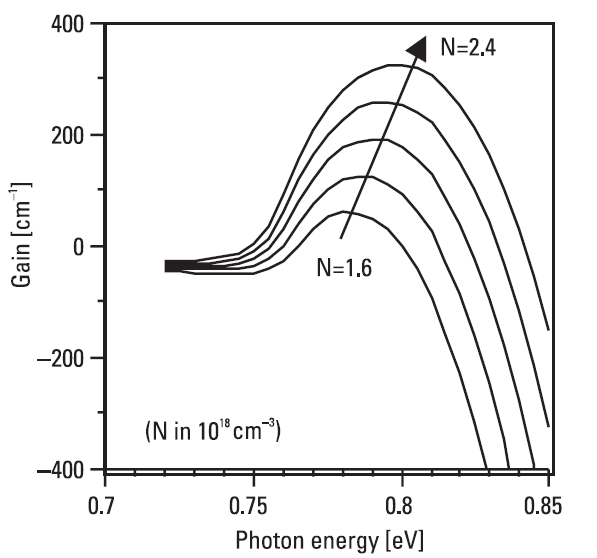
\includegraphics[width=11cm]{./Pictures/fab_bulk_material_gain.png}
	\captionsetup{justification=centering}
	\caption{体材料InGaAsP中增益与载流子密度和光子能量之间的关系\cite{morthier2013handbook}}
	\label{bulk_material_gain}
\end{figure}

\subsection{半导体激光器中的弛豫振荡}
半导体激光器的幅度调制、频率调制可以通过求解载流子密度速率方程和光子密度速率方程得到,在求解过程中,我们假设激光器处于单模工作状态,忽略自发发射,因为与受激辐射的光子数相比,自发辐射的光子数很少。在电流调制的作用下,激光器内的载流子密度$N$、光子密度$S$、电流密度$J$可以表示为:

\begin{equation}
\label{current_modulation}
\begin{array}{l}
N(t) = N_{0}+ Re(N_{1}e^{j\Omega t})\\
N(t) = N_{0}+ Re(N_{1}e^{j\Omega t})\\
N(t) = N_{0}+ Re(N_{1}e^{j\Omega t})
\end{array}
\end{equation}

将其代入载流子密度速率方程\ref{carrier_density_rate_equation}和光子密度速率方程\ref{photon_density_rate_equation},我们只考虑线性项,则可以得到小信号调制下的方程:

\begin{equation}
\label{small_modulation}
\begin{array}{l}
(j\Omega + \dfrac{1}{\tau_{d}} + \dfrac{\partial G}{\partial N}S_{0})N_{1} = \dfrac{J_{1}}{qd} - (G+\dfrac{\partial G}{\partial S}S_{0})S_{1}\\
(j\Omega - \dfrac{\partial G}{\partial S}S_{0})S_{1} = (\dfrac{\partial G}{\partial N}-\dfrac{\partial \gamma}{\partial N})S_{0}N_{1}
\end{array}
\end{equation}

其中,我们忽略了增益的波长相关性,$\tau_{d} = \dfrac{1}{A+2BN_0 +3CN_0^2}$表示微分载流子寿命。通过公式\ref{small_modulation}容易解得$S_{1}$与$N_{1}$,其中$S_{1}$就对应强度调制的响应,$N_{1}$通过与公式\ref{frequency_carrier_relation}就可以得到频率调制的响应:

\begin{equation}
\label{am_fm}
\begin{array}{l}
S_{1} = \dfrac{(\dfrac{\partial G}{\partial N}-\dfrac{\partial\gamma}{\partial N})S_{0}\dfrac{J_{1}}{qd}}{(j\Omega-\dfrac{\partial G}{\partial S}S_{0})(j\Omega+\dfrac{1}{\tau_{d}}+\dfrac{\partial G}{\partial N}S_{0})+G(\dfrac{\partial G}{\partial N}-\dfrac{\partial\gamma}{\partial N})S_{0}}\\
\Delta\omega = \dfrac{\alpha}{2}\dfrac{\partial G}{\partial N}\dfrac{(j\Omega+\dfrac{\partial G}{\partial S}S_{0})\dfrac{J_{1}}{qd}}{(j\Omega-\dfrac{\partial G}{\partial S}S_{0})(j\Omega+\dfrac{1}{\tau_{d}}+\dfrac{\partial G}{\partial N}S_{0})+G(\dfrac{\partial G}{\partial N}-\dfrac{\partial\gamma}{\partial N})S_{0}}
\end{array}
\end{equation}

从中,我们可以看到强度调制与频率调制的响应与调制的频率相关,且其相互之间通过载流子的动态过程相互耦合,故对激光器进行强度调制时,往往也伴随着频率调制(啁啾现象),这也是限制直调激光器在光通信系统中使用的因素之一。为了减小啁啾现象,可以通过减小线宽增强因子$\alpha$来实现。多量子阱激光器相比于体材料有更小的线宽增强因子,故其更适用于制作直调激光器。图\ref{laser_amfm_response}展示了典型的强度调制和频率调制的频率响应图。

\begin{figure}[htb]
	\centering
	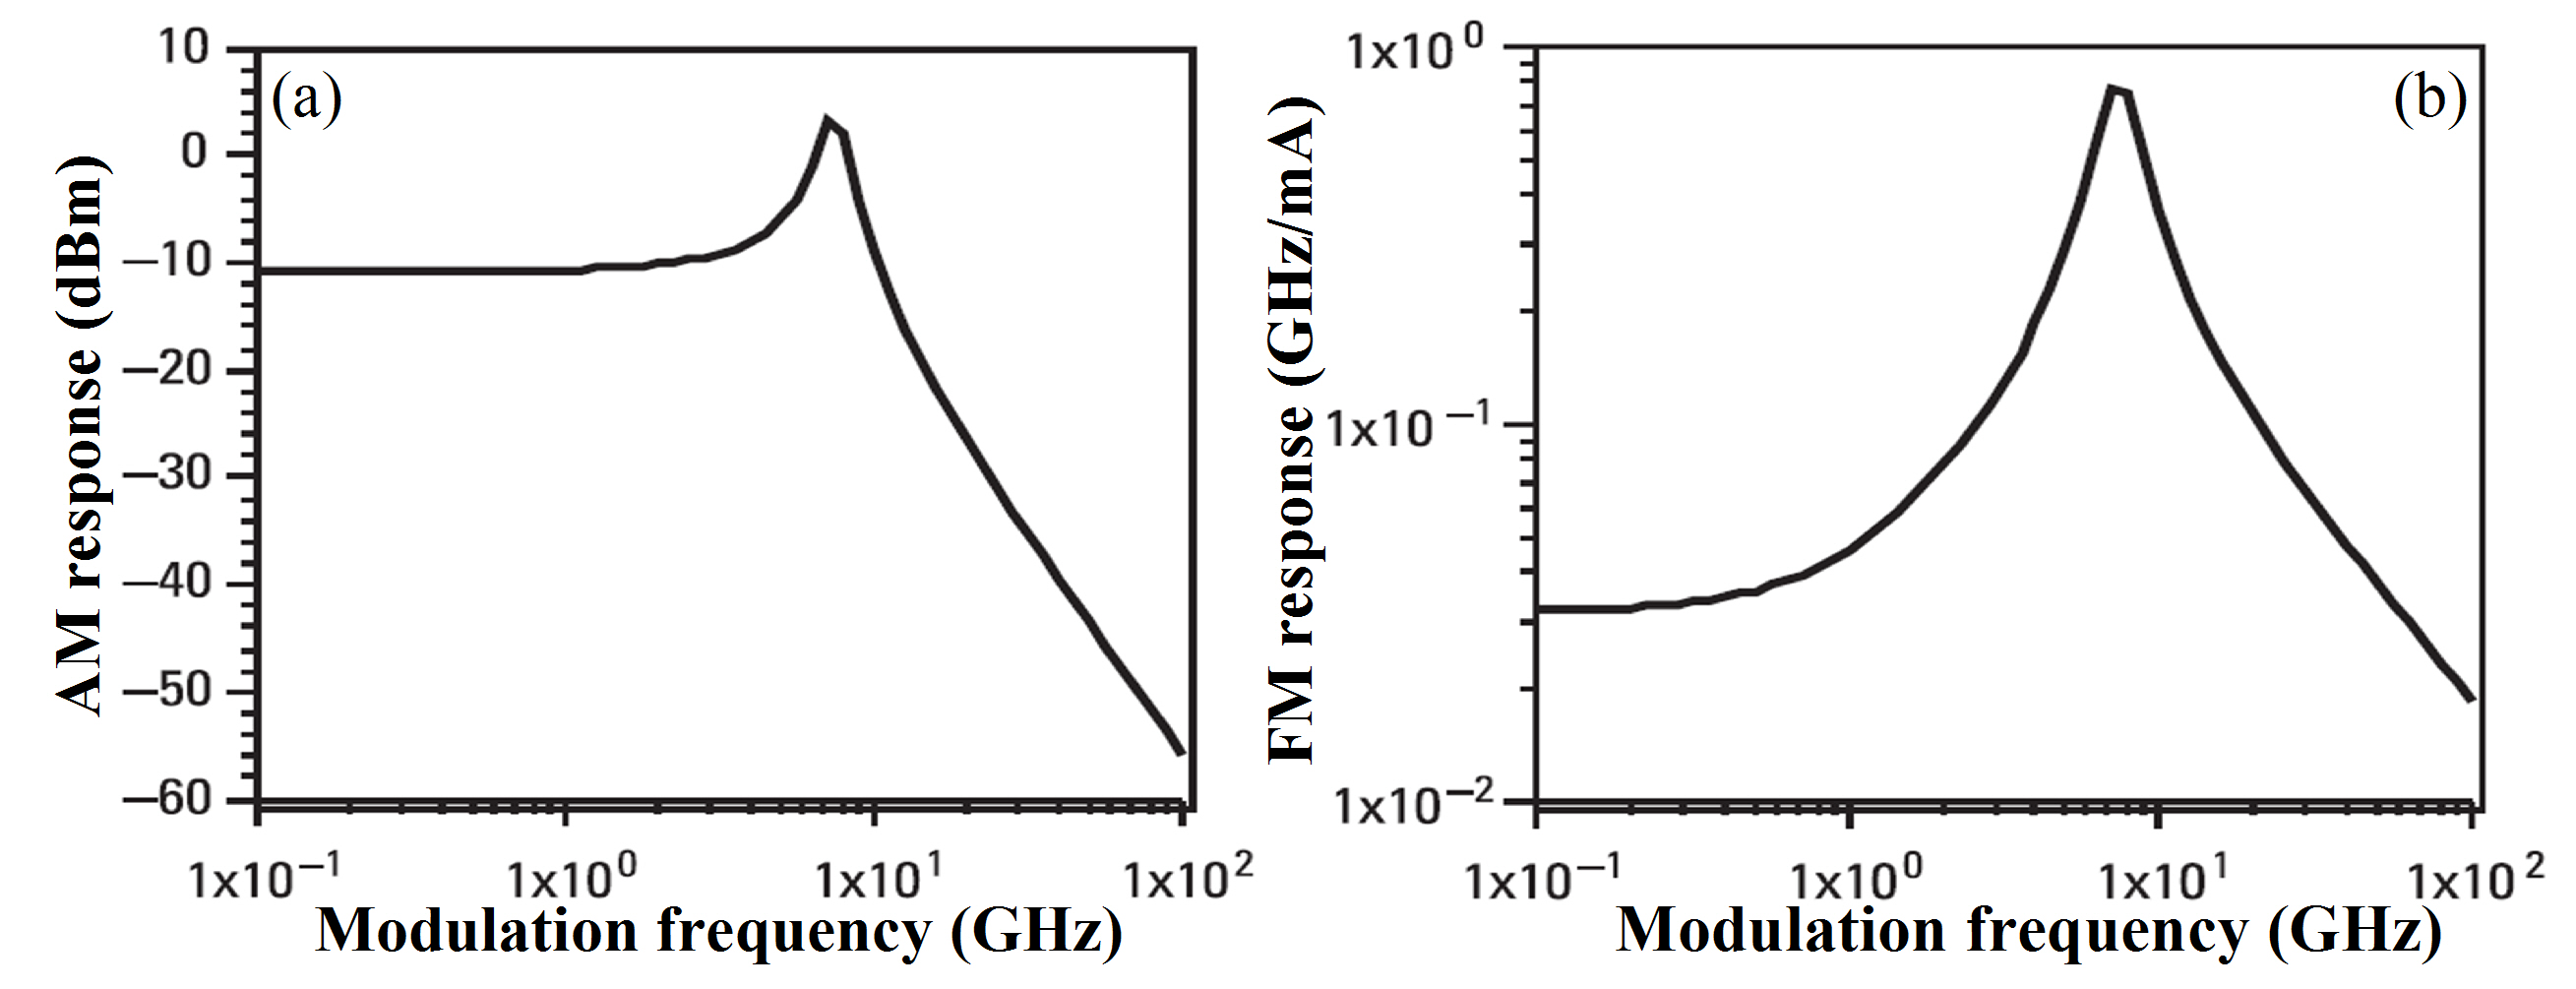
\includegraphics[width=16cm]{./Pictures/laser_amfm_response.jpg}
	\captionsetup{justification=centering}
	\caption{典型的强度调制和频率调制的频率响应;(a)幅度调制响应;(b)频率调制响应\cite{morthier2013handbook}}
	\label{laser_amfm_response}
\end{figure}

从中我们可以看到明显的谐振现象,一般把这种在半导体激光器中,由于驱动电流调制所产生的谐振现象称为激光器的驰豫振荡,其谐振频率$f_{r}$与阻尼系数$\theta$可由公式\ref{relaxation_oscillation}得到,其所对应的物理过程为载流子与光子之间通过受激辐射和受激吸收这两个过程进行能量交换。在稳态条件下,调制电流注入一部分载流子,使得此时激光器的增益会大于损耗,受激辐射就会产生更多的光子。但是随着光子数的增多消耗了激光器内的载流子,使其浓度下降,导致激光器的增益小于损耗,然后光子数又会减少,受激辐射就会减弱,使得载流子浓度又得以升高,如此往复。由于弛豫振荡现象的存在,导致激光器在调制的过程中当调制频率大于弛豫振荡的频率时,信号会出现畸变,这就限制了激光器调制速率的上限。

\begin{equation}
\label{relaxation_oscillation}
\begin{array}{l}
(2\pi f_{r})^{2} = G_{th}(\dfrac{\partial G}{\partial N}-\dfrac{\partial\gamma}{\partial N})S_{0} \approx \dfrac{\partial G}{\partial N}\dfrac{I-I_{th}}{qV_{act}}\\
\theta = \dfrac{1}{\tau_{d}} + \dfrac{\partial G}{\partial N}S_{0}+\dfrac{\partial G}{\partial S}S_{0}
\end{array}
\end{equation}

从公式\ref{relaxation_oscillation}中我们可以看到,弛豫振荡频率与阻尼系数都随着稳态时的光子密度和微分增益的增加而增加,因为其可以加快光子与电子之间能量交换的速率。而且,通过增加模式限制因子,缩小有源区的体积也可以增加驰豫振荡的频率,通常谐振频率处于几个GHz到10几个GHz之间。

\subsection{耦合模理论}

DFB激光器是一个非常复杂的系统,其包括电、光、热之间的非线性耦合过程。想要将所有过程都详细地讨论是不现实的,但是过于简化的模型也不适用于解释DFB激光器的各种物理现象,耦合模理论提供了这样一种平衡,其可以用来分析DFB激光器中载流子密度与光子密度的分布问题。

DFB激光器中的光场可以表示成正向传输的光场$F(z)$和反向传输的光场$B(z)$之和:
\begin{equation}
\label{field_sum}
E(z) = F(z)exp(i\beta z) + B(z)exp(-i\beta z)
\end{equation}
其中,$\beta$为模式的传播常数。正向传输的光场$F(z)$和反向传输的光场$B(z)$通过DFB光栅会互相耦合,耦合系数$\kappa$与光栅的折射率的变化量$\Delta n$成正比,耦合方程可以写为:
\begin{equation}
\label{coupling_dfb1}
\dfrac{dF(z)}{dz} = (\gamma-j\Delta \beta)F(z)-j\kappa B(z)
\end{equation}
\begin{equation}
\label{coupling_dfb2}
\dfrac{dB(z)}{dz} = -(\gamma-j\Delta \beta)B(z)-j\kappa F(z)
\end{equation}
其中,$\gamma$表示模式的增益,$\Delta\beta$表示传播常数与布拉格波矢之间的失谐因子:
\begin{equation}
\label{delta_beta}
\Delta\beta = \dfrac{2\pi n_{eff}}{\lambda} - \dfrac{\pi}{\Lambda}
\end{equation}
其中,$\Lambda$为布拉格光栅的周期。

有了$F(z)$和$B(z)$的耦合方程之后,结合$z=z_0$处给定的初始条件,可以求得任意坐标处的值,其结果可以表示为:
\begin{equation}
\label{coupling_result}
\left[\begin{matrix}
F(z) \\
B(z)
\end{matrix}\right] = \left[\begin{matrix}
cosh(Sz)+\dfrac{\gamma-j\Delta\beta}{S}sinh(Sz) & -\dfrac{j\kappa}{S}sinh(Sz) \\ 
-\dfrac{j\kappa}{S}sinh(Sz) & cosh(Sz)-\dfrac{\gamma-j\Delta\beta}{S}sinh(Sz)
\end{matrix}\right]\left[\begin{matrix}
F(z_0)\\
B(z_0)
\end{matrix}\right]
\end{equation}
其中,$S^2 = \kappa^2+(\gamma-j\Delta\beta)^2$。该矩阵也叫做$z$与$z_0$之间的传输矩阵$T$,如果我们考虑DFB激光器两边都镀上减反膜,即两边的反射率为零。并且让$z=L$,$z_0=0$,利用边界条件可以求得$T_{22}=0$,即:
\begin{equation}
\label{boudary_condition_result}
SLcoth(SL) - \gamma L + j\Delta\beta L = 0
\end{equation}

通过数值方法求解公式\ref{boudary_condition_result}可以得到不同耦合系数下模式增益$\gamma L$与$\Delta\beta L$之间的关系如图\ref{fab_stopband}(a)所示,从中可以看出,对于中心无$\lambda/4$相移的DFB激光器来说,其在失谐因子$\Delta\beta L=0$处即布拉格波长处没有模式,其两个一阶模式对称分布在布拉格波长两边,它们之间的距离称之为DFB激光器的阻带宽度,可以反映激光器的耦合强度,耦合强度越强,阻带宽度也就越大,对于没有增益与损耗的布拉格光栅来说,其关系如公式\ref{stopband_coupling_coefficient}所示:
\begin{equation}
\label{stopband_coupling_coefficient}
\Delta\lambda = \dfrac{\lambda_\beta^2}{\pi n_{eff}L}\sqrt{(\kappa L)^2+\pi^2}
\end{equation}

由于这两个一阶模式拥有相同的阈值增益,故该类DFB激光器往往具有多模特性。这两个一阶模式的简并可以通过图\ref{fab_lambda_4_explanation}进行解释,观察$z_1$与$z_2$处反射波的相位叠加,由于光场经过$\Lambda/2$距离的传输,相位变化为$\pi/2$,所以每个光栅界面反射的光波相位差在$0$和$\pi$之间变化,$z_1$与$z_2$处的光场叠加将处于干涉相长状态。如果DFB光栅中心无$\lambda/4$的相移,则经过$\Lambda/2$距离的传输,相位差将变为$(2p+1)\pi$,其中$p$为整数,故在布拉格波长处无模式存在。

\begin{figure}[htb]
	\centering
	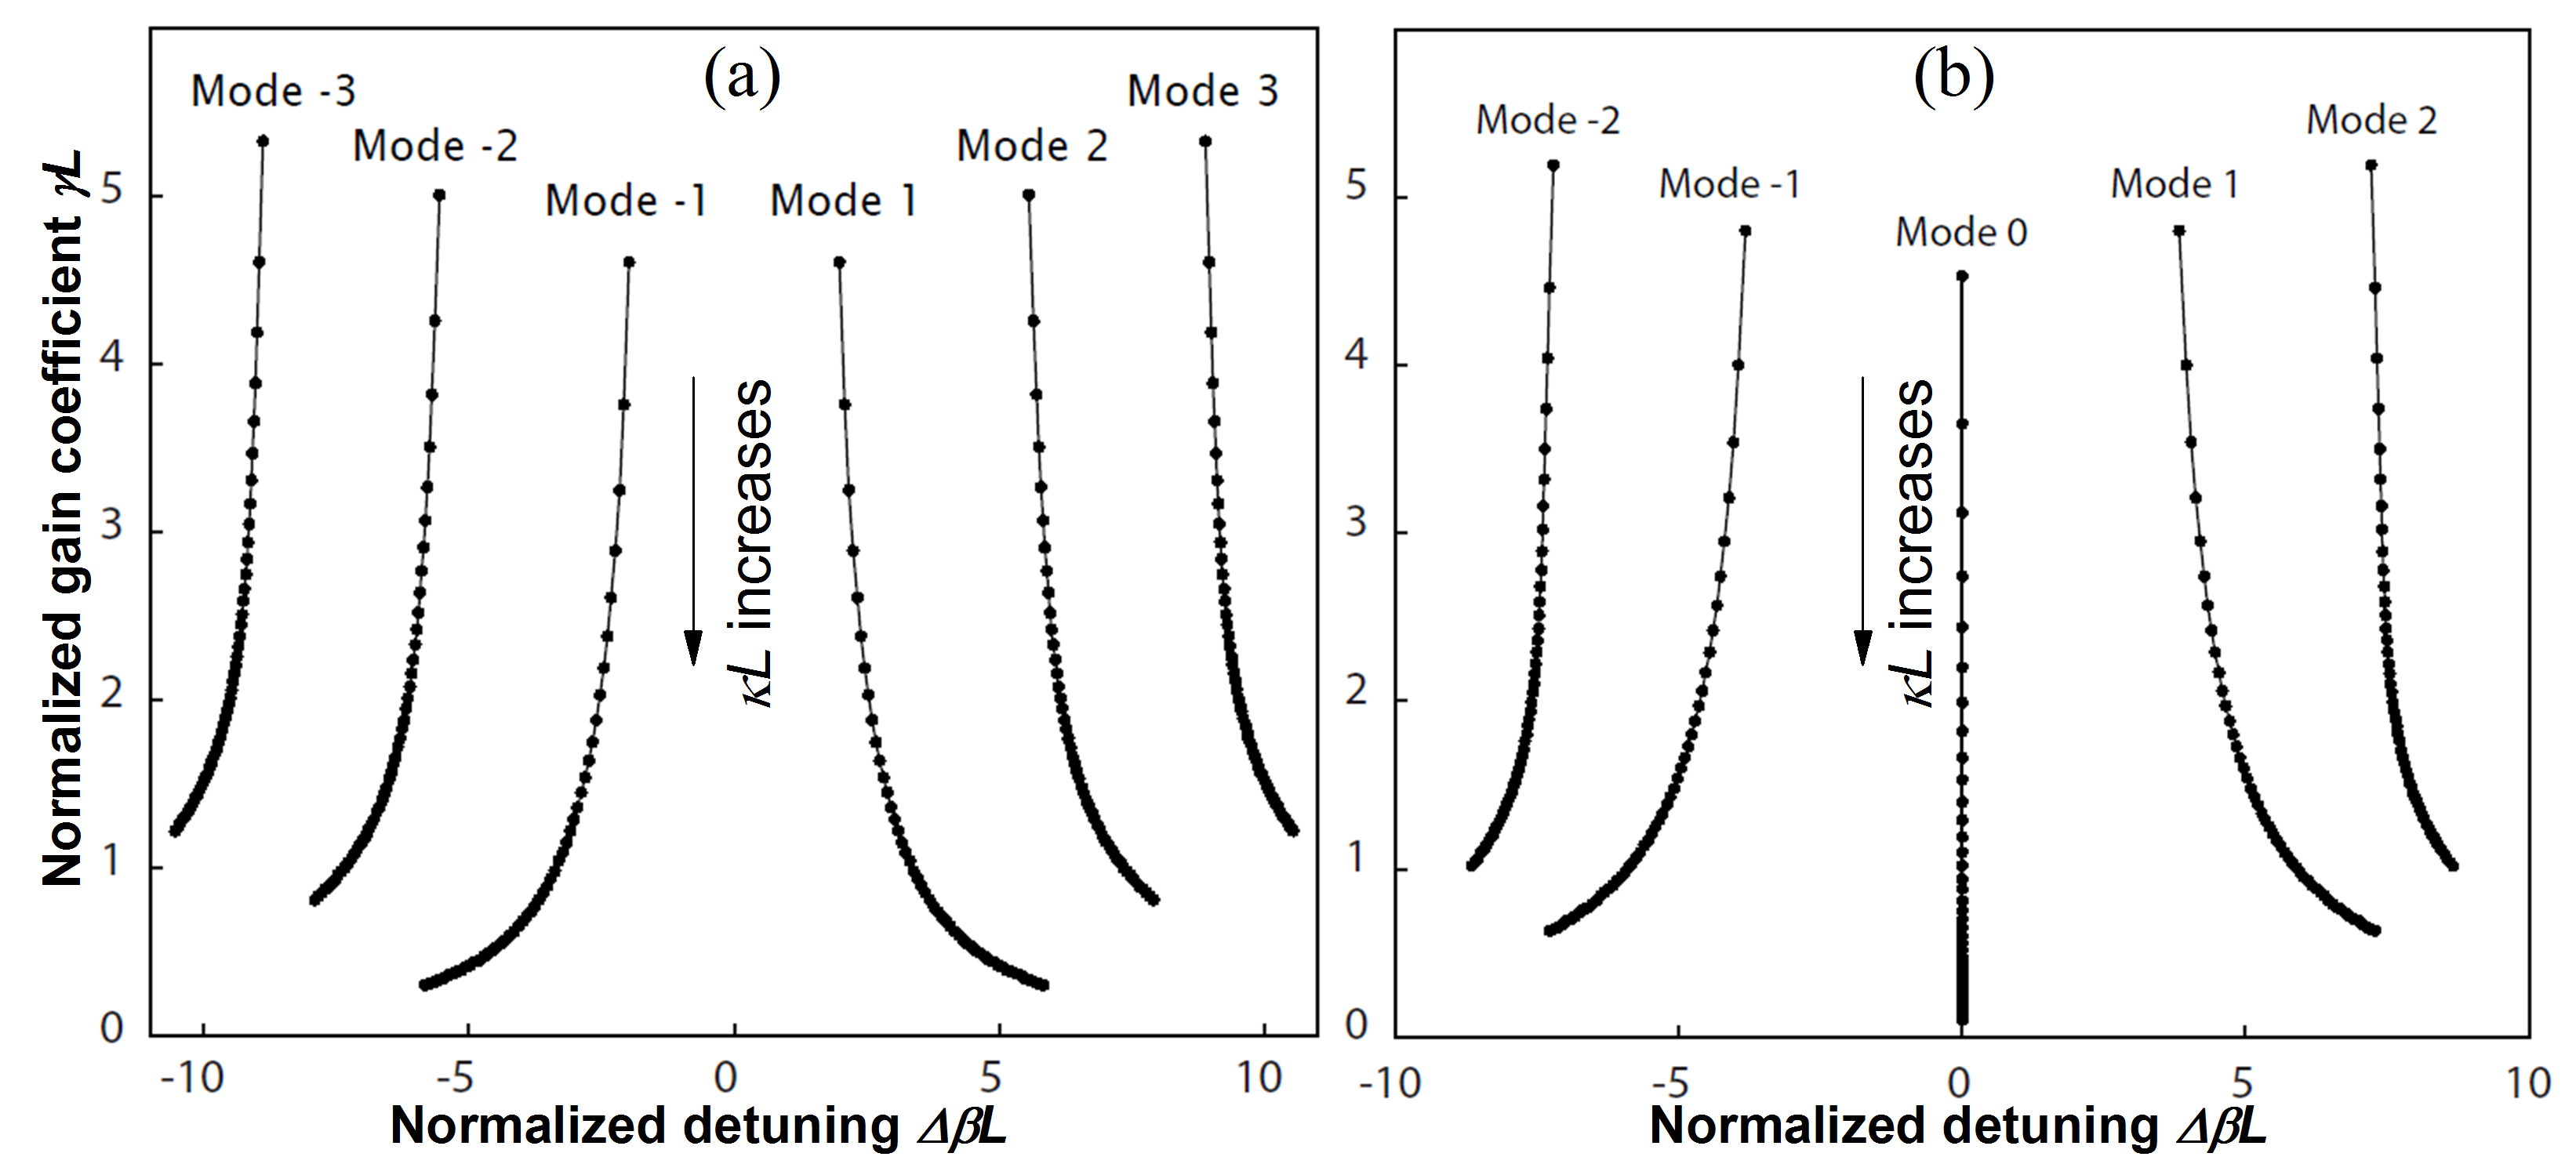
\includegraphics[width=16cm]{./Pictures/fab_stopband.jpg}
	\captionsetup{justification=centering}
	\caption{不同归一化耦合强度$\kappa L$下,归一化阈值增益与归一化失谐因子之间的关系,(a)中心无$\lambda/4$相移的DFB激光器;(b)中心有$\lambda/4$相移的DFB激光器\cite{huybrechts2010digital}}
	\label{fab_stopband}
\end{figure}

\begin{figure}[htb]
	\centering
	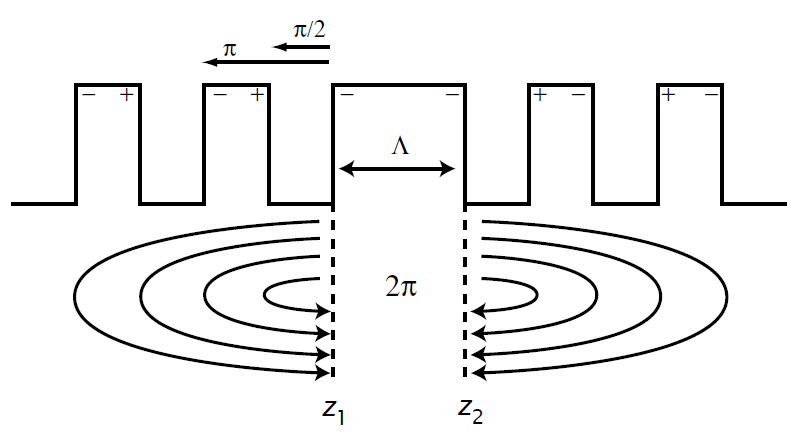
\includegraphics[width=12cm]{./Pictures/fab_multimode_explanation.png}
	\captionsetup{justification=centering}
	\caption{DFB光栅中央处$\lambda/4$相移作用的物理解释\cite{morthier2013handbook}}
	\label{fab_lambda_4_explanation}
\end{figure}

要解决这个问题,可以在DFB光栅中心加入$\lambda/4$的相移,此时就可以将$z_1$与$z_2$处的光场增加额外的$\pi$相位,从而消除模式简并。添加$\lambda/4$的相移之后,DFB激光器的传输矩阵可以变为$T(L/2)T(\Lambda/2)T(L/2)$,公式\ref{boudary_condition_result}变为:
\begin{equation}
\label{boudary_condition_result2}
SLcoth(SL/2) - (\gamma L - j\Delta\beta L \pm \kappa L) = 0
\end{equation}
利用数值方法求解公式\ref{boudary_condition_result2}得到不同耦合系数下模式增益$\gamma L$与$\Delta\beta L$之间的关系如图\ref{fab_stopband}(b)所示,此时在布拉格波长处的模式的阈值增益最小,故我们可以知道,两边镀减反膜且中心加入$\lambda/4$相移的DFB激光器可以实现单模激射。



\section{光子器件基本制作工艺}
得益于SOI平台的高折射率差,硅基光电子器件的特征尺寸在亚微米量级,最常见的单模波导,其宽度为500~$nm$,如果采用狭缝结构的波导,其狭缝的宽度则只有100~$nm$左右。对于片上的一阶布拉格反射镜,其周期在400~$nm$左右,所以其单个光栅的尺寸也在200~$nm$左右,对于一维光子晶体纳米梁腔,其特征尺寸更小。普通的接触式光刻已经无法满足如此高的加工精度要求,所以制作这类器件常常需要使用电子束曝光(electro-beam lithography, EBL)来完成器件的制作。基于电子束曝光的硅基光子器件制作过程通常包括SOI芯片的清洗与匀胶、电子束曝光与显影、刻蚀等工艺流程,下面主要介绍以上主要工艺流程。

\subsection{SOI芯片的清洗与匀胶}
我们以220~$nm$~SOI(SOITEC Inc.)芯片为例,来介绍硅光子学器件的基本工艺流程。解理完合适大小的SOI芯片后,一般为1.5~$cm$~$\times$~1.5~$cm$,方便工艺过程中用镊子进行操作。解理完之后芯片表面一般如图\ref{fab_surface}所示,可以看到SOI芯片表面会吸附很多有机物等杂质,所以需要对其进行清洗。
\begin{figure}[htb]
	\centering
	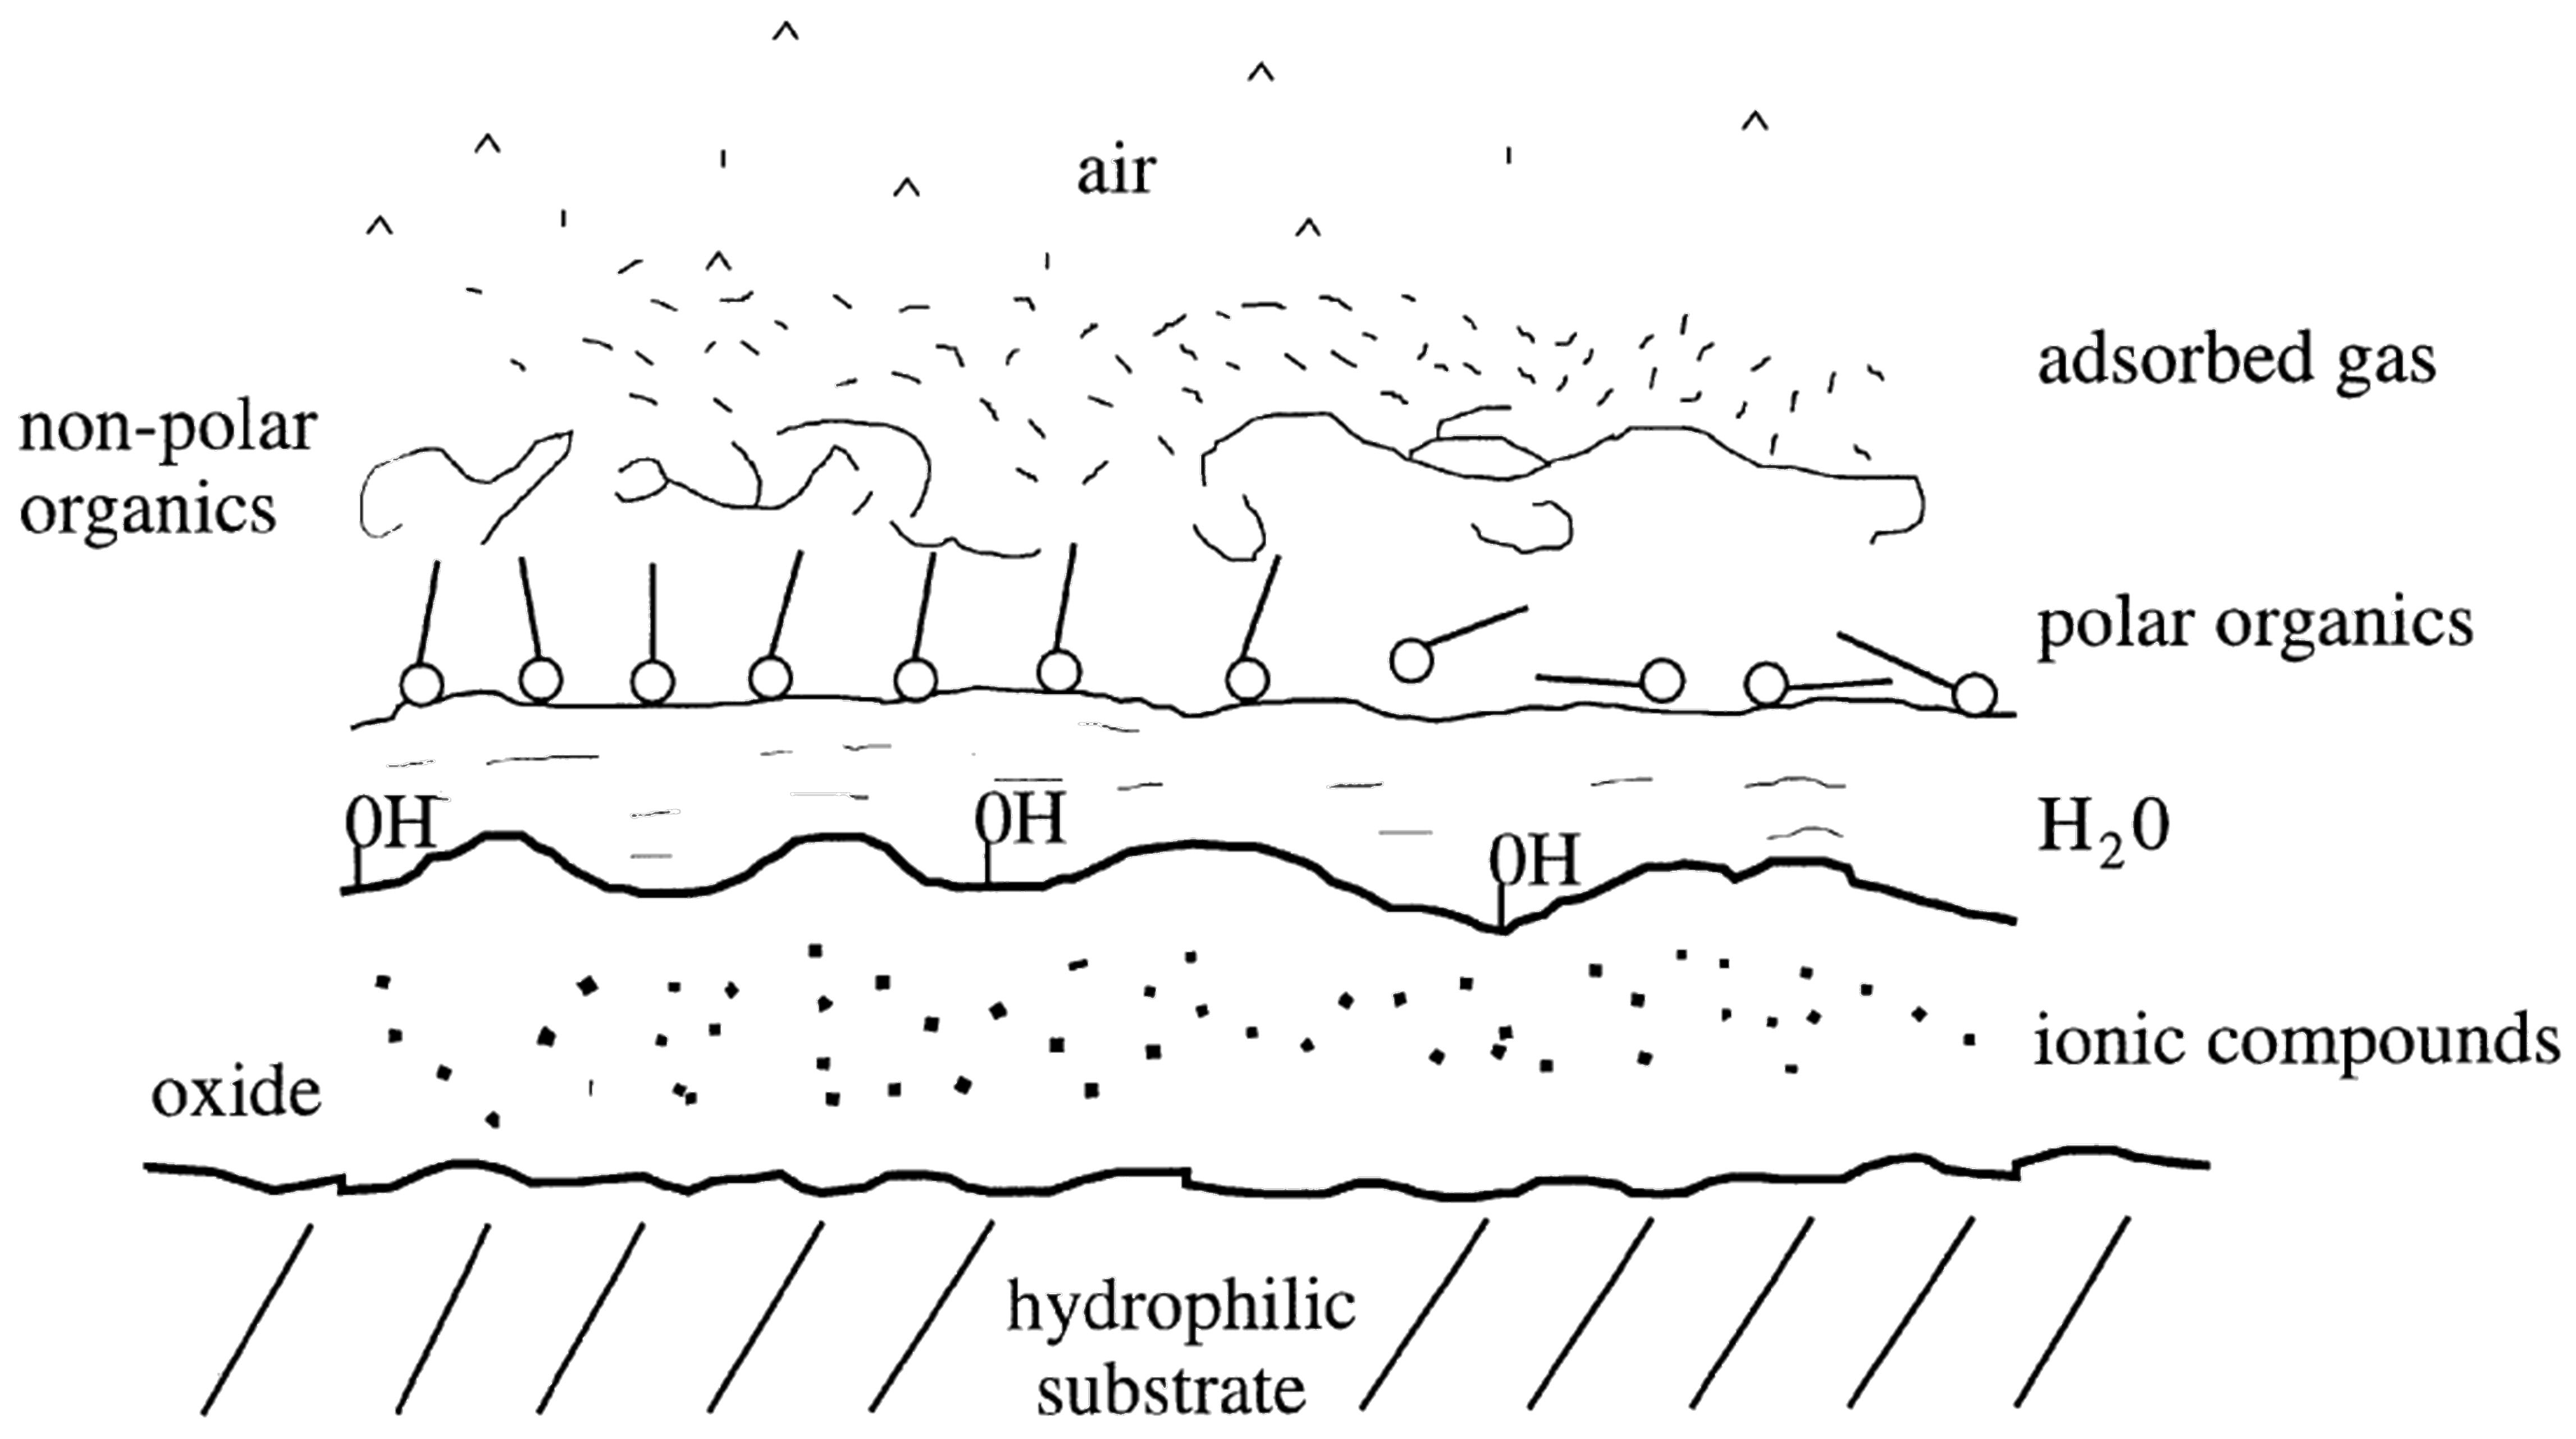
\includegraphics[width=14cm]{./Pictures/fab_surface.jpg}
	\captionsetup{justification=centering}
	\caption{亲水表面通常会吸附的物质\cite{plossl1999wafer}}
	\label{fab_surface}
\end{figure}

主要的清洗步骤为:
\begin{enumerate}[(1)]
	\item 
	用氮气枪吹扫SOI芯片表面,去除可能因解理时落在上面的硅小颗粒,不宜用较强的气流,否则硅小颗粒有可能划伤SOI芯片的表面。
	\item 
	由于SOI芯片表面往往会吸附有机物杂质,故需要用丙酮、甲醇、异丙醇分别超声清洗5~$min$,去除有机物杂质。
	\item 
	将SOI芯片用浓H\SB{2}SO\SB{4}:H\SB{2}O\SB{2}=1:1(体积比)的食人鱼溶液浸泡2~\~{}3小时,该步骤是为了去除表面的残留有机物。用其他比例也是可以的,它们还是可以被叫做食人鱼溶液。浸泡食人鱼溶液之前一定要将前一步有机物去除干净,只允许有非常少的残留,否则有可能会引起爆炸。
	\item 
	经过食人鱼溶液处理过后的SOI表面会被羟基(-OH)化,芯片表面会变成亲水性。由于我们使用的电子束光刻胶一般都属于有机试剂,故经过食人鱼溶液处理的SOI芯片直接进行匀胶的话,胶与芯片表面的粘附性往往不够好,故需要将SOI芯片在氢氟酸缓冲液(buffered oxide etch, BOE)中浸泡10~$s$左右,以去除表面的羟基(-OH),其组成为NH\SB{4}F:HF~=~6:1。随后用去离子水清洗干净之后,置于热板上烘干。
\end{enumerate}

完成以上清洗步骤之后,就可以准备将电子束光刻胶(又可以称为电子束抗蚀剂)旋涂到SOI芯片表面。对于电子束光刻胶,可以分为正胶和负胶,对于正胶来说,经过电子束曝光使得光刻胶中原本存在的交联断裂,在之后的显影过程中容易被溶解掉;对于负胶来说,电子束曝光使得光刻胶中的小分子发生交联,在之后的显影过程中不容易被溶解。实验室常用的正胶有聚异丁烯酸甲酯(Polymethylmethacrylate, PMMA),ZEP 520A(主要由$\alpha$-氯代甲基丙烯酸酯和$\alpha$-甲基苯乙烯的共聚物组成),负胶有ma-N2400系列等。几种常用的电子束光刻胶使用参数如表\ref{ebeamresist}所示:

\begin{table}[htb]
	\zihao{5}
	\captionsetup{justification=centering}
	\caption{实验室常用的三种电子束光刻胶及其各项参数}
	\label{ebeamresist}
	\centering
	\begin{tabular}[t]{cccccccc}
		\hline
		\textbf{光刻胶} & \textbf{转速(r/min)}  & \textbf{前烘} & \textbf{显影(s)} & \textbf{定影(s)} & \textbf{坚膜} & \textbf{剂量(30kV)} \\
		\hline
		PMMA & 4000 &  180$^{\circ}$C~10~$min$ & 35 & 35 & 90$^{\circ}$C~10~$min$ & 300 \\
		\hline
		ZEP 520A & 6000 &  180$^{\circ}$C~10~$min$ & 40 & 60 & 120$^{\circ}$C~10~$min$ & 95 \\
		\hline
		ma-N 2403 & 4000 &  90$^{\circ}$C~90~$s$ & 150 & null & 110$^{\circ}$C~40~$min$ & 130 \\
		\hline
	\end{tabular}
\end{table}

匀胶是将液态粘稠的光刻胶通过快速旋转,借助离心力均匀地涂覆到SOI芯片上的过程,光刻胶的厚度可以根据光刻胶浓度与转速控制,达到想要的厚度。决定匀胶厚度时,常常需要考虑到光刻胶与硅的刻蚀比,对于PMMA来说,其与硅的刻蚀比在1:1\~{}2左右,即刻蚀1~$nm$~PMMA,可以刻蚀1\~{}2~$nm$的硅。对于ZEP 520A,刻蚀比可以达到1:4,故其可以用来制作刻蚀深度更大的器件。图\ref{fab_spinner}为实验室所使用的匀胶机。

\begin{figure}[htb]
	\centering
	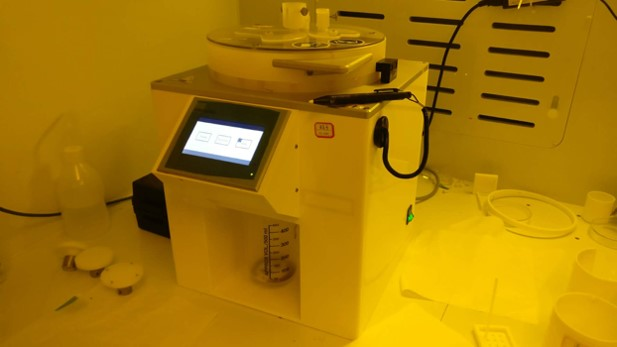
\includegraphics[width=12cm]{./Pictures/fab_spinner.jpg}
	\captionsetup{justification=centering}
	\caption{SUSS Micro Tec 公司的Labspin6匀胶机}
	\label{fab_spinner}
\end{figure}
匀胶的具体过程如下:
\begin{enumerate}
	\item 
	将SOI芯片置于匀胶机吸盘中央并使吸盘处于抽真空状态,使得芯片被固定住以防在高速旋转式被甩出去,污染芯片。此步往往需要借助蓝膜增加气密性。
	\item 
	设置好匀胶机的参数,一般包括前转和后转,其中前转主要是为了控制开始旋转的加速过程,以便光刻胶能够能够较为快速地分布到整块SOI芯片上,但如果前转速度太快,会导致光刻胶直接被甩飞出去,无法形成均匀的覆盖。后转是为了让SOI芯片上的各处光刻胶厚度尽量均匀一致。以PMMA 950K 679.04为例,其前转一般为3000~rpm~3~$s$,后转为4000~rpm~59~$s$。
	\item 
	将适量光刻胶滴于SOI芯片表面,盖上保护罩,点击开始按钮。
	\item 
	匀胶结束后关闭真空,将SOI芯片从匀胶机中取下,并清洗匀胶机。
\end{enumerate}

从匀胶机上取下的带有光刻胶的芯片还不能直接用于电子束曝光,因为刚匀好的光刻胶中含有一定量的挥发性溶剂,该溶剂是为了光刻胶能够更好的旋涂而加入的,这就需要前烘这一步工艺。去掉溶剂的目的在于,保证光刻胶性能的稳定,提高胶的扛刻蚀能力。

\subsection{电子束曝光}

制作硅基光电子集成器件时,影响器件性能最主要的决定因素便是光刻。一方面光刻的质量影响了波导线条的光滑程度,进而影响了器件的损耗特性,另一方面,光刻的最小分辨率也决定了器件所能达到的最小尺寸。相较于传统的光刻,其分辨率受到光场衍射的限制,最小尺寸为所用曝光波长的一半左右。对于电子束曝光来说,根据微观粒子波粒二象性,电子也可以看成是一种物质波,其波长可以由德布罗意物质波波长公式计算得到:
\begin{equation}
	\lambda = \dfrac{h}{p}	
\end{equation}
其中,普朗克常数$h=6.625\times10^{-34}J\cdot s$,$p$为电子的动量。根据上式可以算出,当电场加速电压为30kV时,电子的波长约为0.007~$nm$。但这并不意味着电子束曝光可以达到这样的精度,电子束曝光的精度还受到电子枪的放大倍率、电子束透镜的球差、色差(不同能量的电子聚焦能力不同)、衍射效应等因素的限制\cite{rai1997handbook}。对于我们实验室的电子束曝光系统,如图\ref{fab_ebl},分辨率可以到5~$nm$。

\begin{figure}[htb]
	\centering
	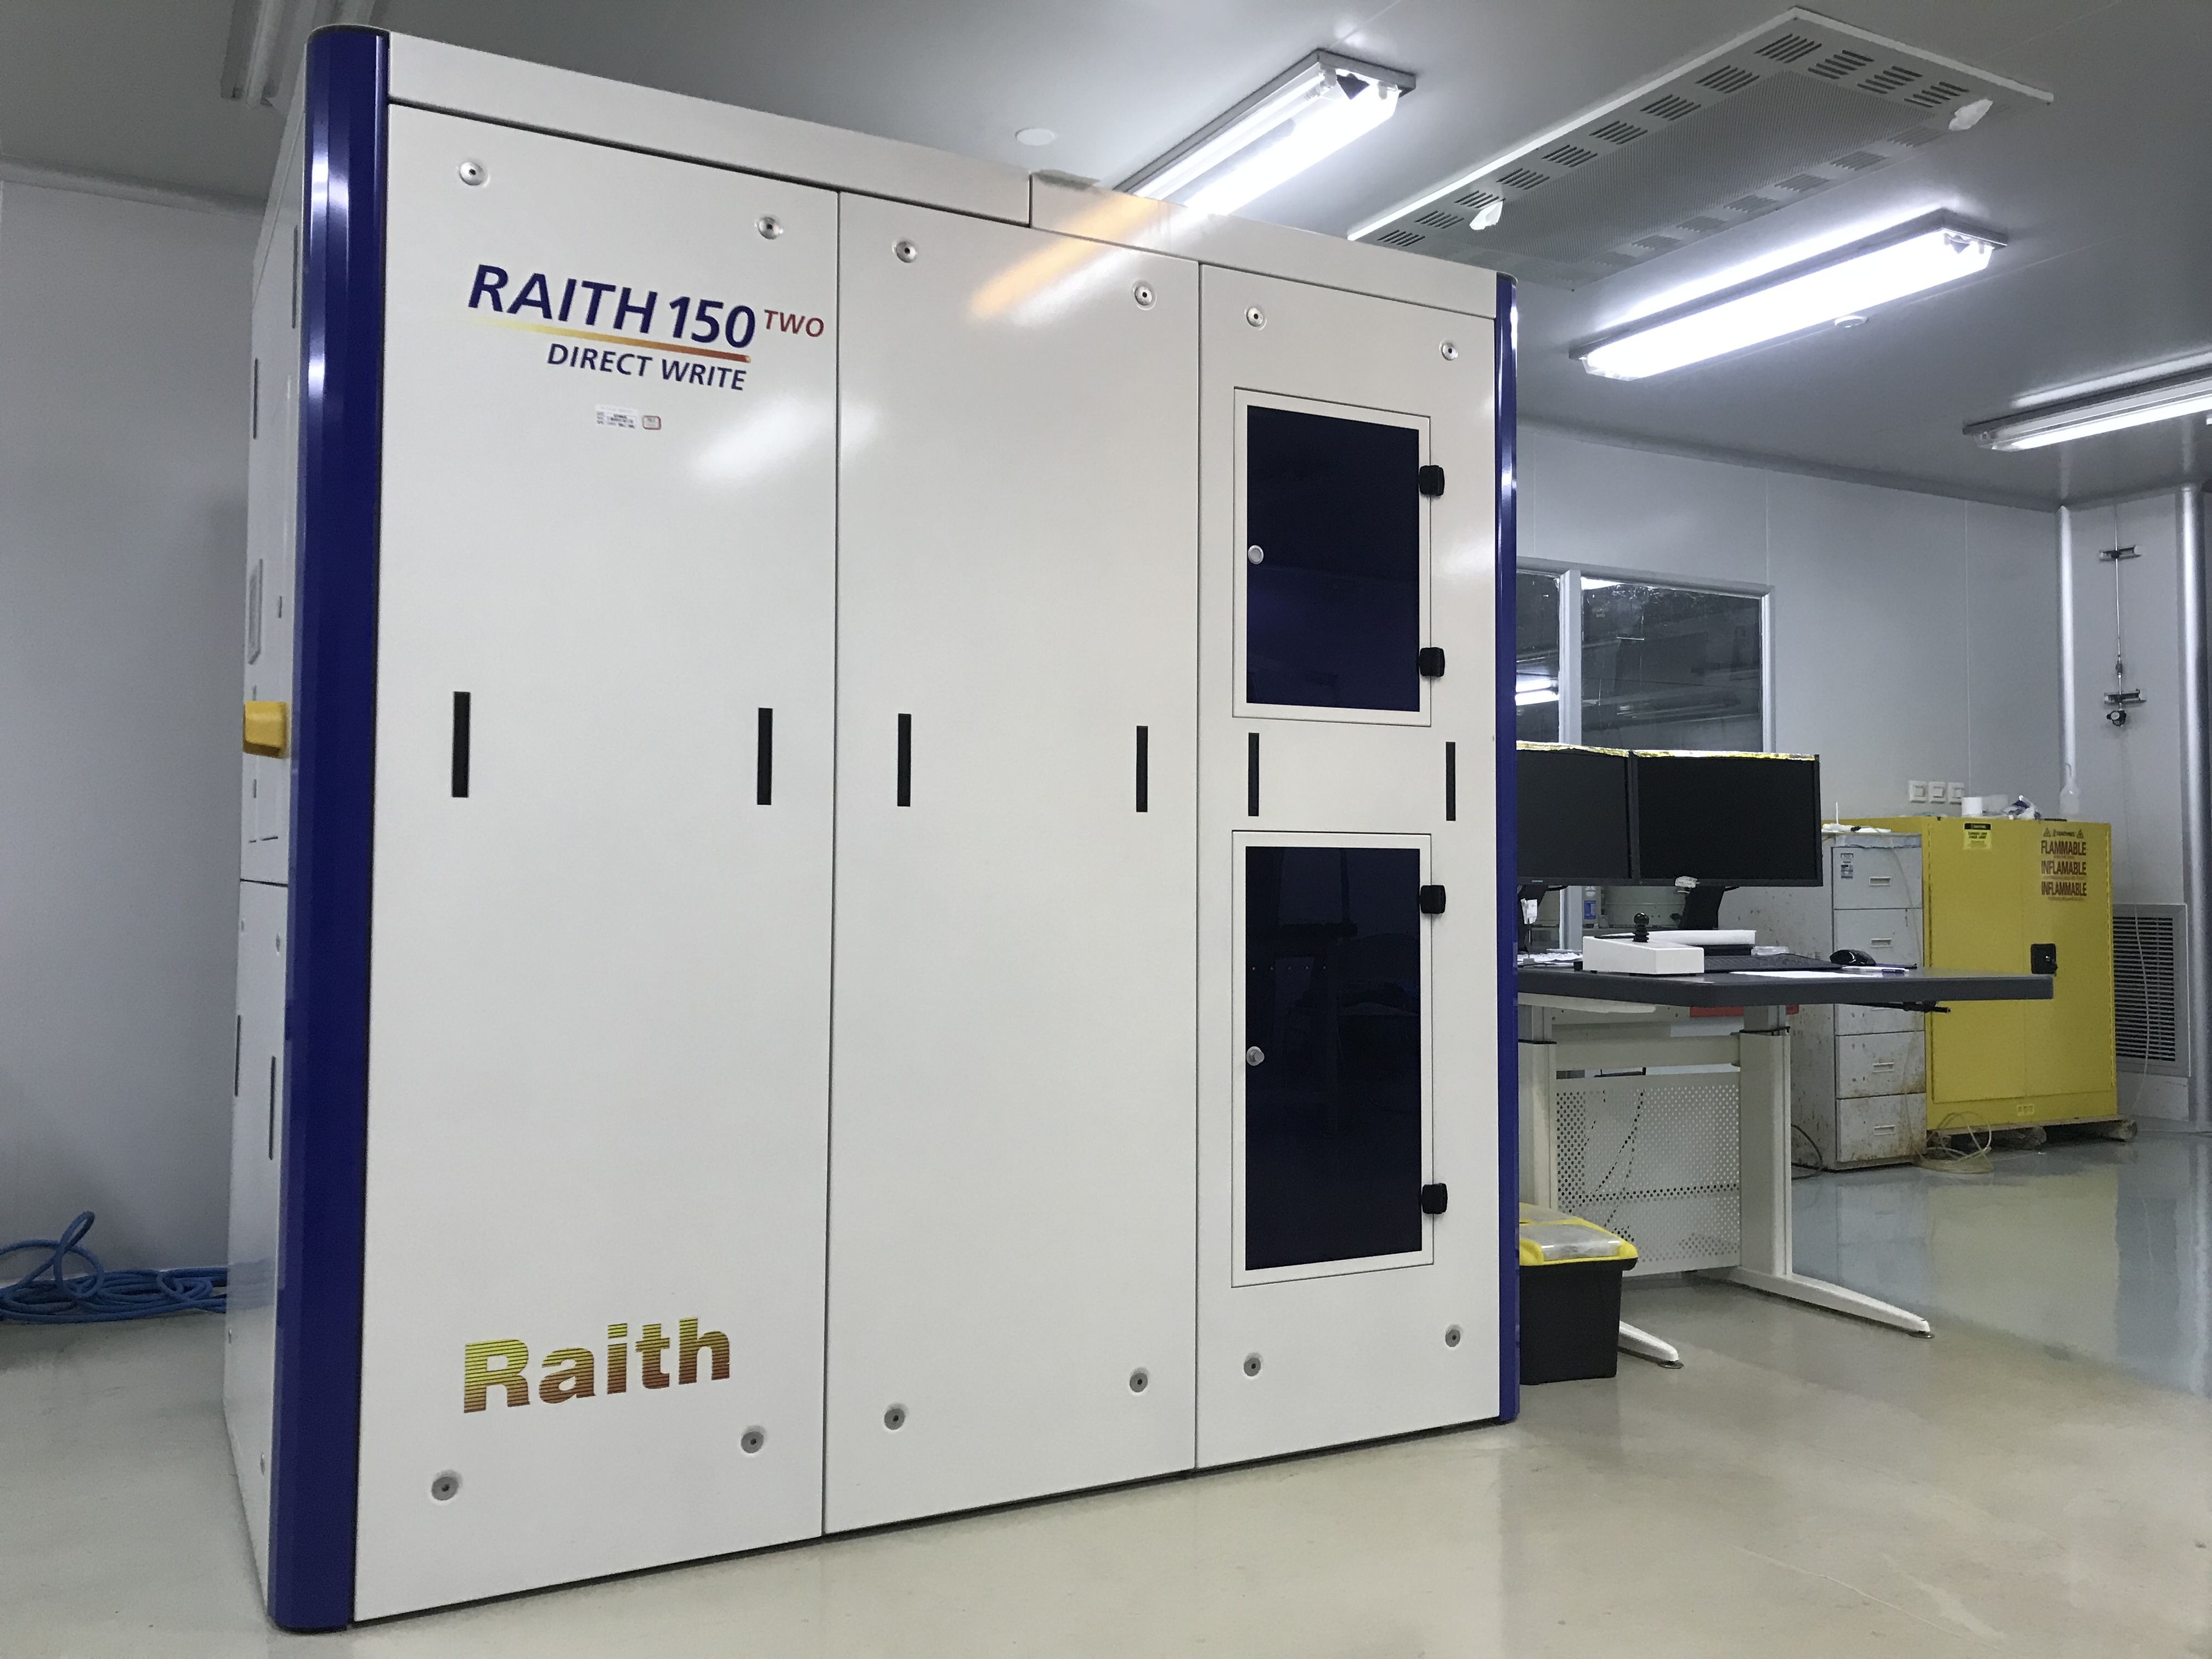
\includegraphics[width=12cm]{./Pictures/fab_ebl.jpg}
	\captionsetup{justification=centering}
	\caption{RAITH 150\SP{TWO}电子束曝光系统}
	\label{fab_ebl}
\end{figure}

我们以PMMA为例介绍电子束曝光过程中的注意事项,我们重点需要关注三个参数:加速电压、电子束光阑孔径和曝光剂量。加速电压主要决定了电子束能量的大小,加速电压越大,电子束的速度也会越大,在轰击样品表面时,越不容易发生大角度散射,故分辨率就会越高。本文后续实验所使用的Raith 150\SP{TWO}最大的加速电压为30~kV。电子束孔径主要控制曝光时电子束电流的大小,电子束孔径越大,则曝光时电子束的电流也就越大。对于同样的曝光图形,电子束孔径越大,曝光的时间就越短。但是电子束孔径增大时,对应的电子束发散程度也会变大,从而会降低分辨率。曝光剂量为单位面积内电子束光刻胶所需要的曝光电荷量,单位为$\mu C/cm^2$,主要由所用电子束光刻胶的性质和其成膜的厚度有关。以PMMA为例,若曝光剂量不足,则曝光区域的光刻胶在显影过程中就无法完全溶解,导致光刻胶的残留。若是曝光剂量过大,则会导致图形尺寸的展宽和侧壁粗糙度的增加。综上,电子束曝光过程的参数都要精心选择,以达到最好的曝光效果。

曝光完成之后,需要进行显影。对于PMMA来说,我们使用的显影液为MIBK(methyl isobutyl ketone) : IPA(isopropyl alcohol)=1:3(体积比)混合溶液,定影液采用IPA,显影参数为:显影35~$s$,定影35~$s$。然后用去离子水将显影液与定影液冲洗干净。

完成显影之后,我们需要对光刻胶进行坚膜处理,坚膜也称为后烘或者硬烘焙,它的作用是蒸发显影、定影过程中残留在基片表面的有机溶液,增强光刻胶与芯片表面的黏附力以及光刻胶的扛刻蚀性能。PMMA的坚膜过程如下:用热板60$^{\circ}$C烘烤5~$min$,再将热板温度设置到90~$^{\circ}$C并保持,继续烘烤几分钟,保证总的坚膜时间为15~$min$。坚膜完成之后,SOI芯片就可以进行后续的刻蚀工艺,将图案从光刻胶转移到芯片上。

\subsection{SOI芯片刻蚀工艺}

刻蚀工艺根据原理的不同,可以分为干法刻蚀与湿法刻蚀两大类。

湿法刻蚀不需要昂贵的设备,操作简单,是早期微纳加工过程中普遍采用的方法。湿法腐蚀硅较为常用的溶液一般有两种:一种是氢氟酸(HF)和硝酸(HNO\SB{3})的混合液,其与硅硅的化学反应式如下:
\begin{equation}
\rm Si+HNO_3+6HF\rightarrow H_2SiF_6+HNO_2+H_2O+H_2
\end{equation}
上式中的主要生成物H\SB{2}SiF\SB{6}与HNO\SB{2}均易溶于水,因此反应可以持续进行。但该方法的一个缺点是氢氟酸与衬底二氧化硅同样会发生反应。

另一种常用的腐蚀液为KOH溶液,其与硅的化学反应式如下:
\begin{equation}
\rm Si+2KOH+H_2O\rightarrow K_2SiO_3+2H_2
\end{equation}
需要特别指出的是,KOH溶液对于不同晶向的硅,其最终腐蚀得到的微槽结构也是不一样的。

湿法腐蚀的缺点在于腐蚀很难形成我们所需要的具有垂直侧壁的波导结构,其加工精度也有限,所以其应用范围也就受到了很大的局限。在对于刻蚀精度和刻蚀质量要求极高的硅基光电子集成器件中,已经极少使用湿法的方式来刻蚀波导器件结构。湿法刻蚀更多的是应用到某些特殊设计需要掏空的器件\cite{liu2016silicon}。

干法刻蚀是指利用化学或物理作用,或者两者同时作用的方法进行刻蚀。在纯化学机制中,主要通过受激等离子体产生的反应原子核自由基和被刻蚀物质之间的化学反应来完成刻蚀,刻蚀气体需要根据不同的刻蚀物材料来选择;在纯物理机制中,采用射频电源将刻蚀气体等离子体化,产生的等离子体高能粒子在电场作用下轰击刻蚀物质,该物理刻蚀方法具有很好的方向性,但缺点在于刻蚀的选择性较差。本文实验采用的是物理性的粒子轰击和化学反应刻蚀相结合的刻蚀方法,该方法又被称作电感耦合等离子体反应粒子刻蚀(Inductively Coupled Plasma Reactive Ion Etching, ICP-RIE)。图\ref{fab_icp}所示为本文所使用的英国STS公司的ICP刻蚀机。

\begin{figure}[htb]
	\centering
	\includegraphics[width=12cm]{./Pictures/fab_icp.jpg}
	\captionsetup{justification=centering}
	\caption{英国STS公司的ICP刻蚀机}
	\label{fab_icp}
\end{figure}

在ICP刻蚀过程中,物理轰击扮演了重要的角色。典型的ICP刻蚀过程包括刻蚀和淀积两类反应。反应物在刻蚀槽的底部和侧壁都会生成有机物保护层,由于等离子体向下轰击的方向性,使得底部的保护层比侧壁的保护层更快地被去掉,从而向下的刻蚀过程能持续进行,最终形成垂直的侧壁。在反应过程中,一般需要两种气体,一种作为刻蚀气体,另一种主要作为侧壁的保护气体。在刻蚀硅时,我们选用SF\SB{6}作为主要刻蚀气体,同时选用C\SB{4}F\SB{8}作为保护气体,合理调节两种气体的比例以及ICP的其他参数,可以使得刻蚀与淀积两种过程平衡,从而得到垂直的波导侧壁。本论文所使用的参数为:腔体温度65$^{\circ}$C,SF\SB{6}气体流量10~$sccm$,C\SB{4}F\SB{8}气体流量5.7~$sccm$,上极板功率为500~$W$,下极板功率为20~$W$,在该参数设定下,硅的刻蚀速率约为1.5~$nm$/s。

刻蚀工艺完成之后,我们需要去除残留的光刻胶和刻蚀残留物,以方便测试或者下一步工艺的顺利进行。去除残胶的常用的方式有如下三种:1、有机溶剂清洗;2、氧气等离子体轰击;3、强氧化剂比如食人鱼溶液清洗。有机溶剂一般采用的是丙酮或者强力去胶剂(N-Methy-Pyrrolidone, NMP),其一般可以溶解部分残胶,但是对刻蚀过程中已经碳化的光刻胶则无能为力。氧气等离子体则利用等离子态的氧气反应活性,与残胶发生氧化反应从而去除残胶。可以使用专门的氧气等离子体设备或者用ICP进行清洗。强氧化剂可以利用其强氧化特性,将残胶分解成CO、CO\SB{2}和H\SB{2}O,从而去除。实际工艺过程中,常常将这三种清洗方法组合使用。

\section{本章小结}
本章首先介绍了平板光波导的概念,并从麦克斯韦方程组出发推导了波动方程,并简要介绍了计算波导模式与光场传输的数值计算方法。然后介绍了DFB激光器的基本原理,包括其速率方程和耦合模理论,并利用速率方程计算得到了激光器的弛豫振荡频率,通过耦合模理论给出了DFB激光器单模激射的条件。最后介绍了本论文所用到的一些基本工艺流程,包括SOI芯片的清洗与匀胶,电子束曝光,刻蚀,并简要分析了其中的参数对工艺的影响。











